\documentclass[12pt, a4paper, reqno]{amsart}
\usepackage[slovene]{babel}
\usepackage[T1]{fontenc}
\usepackage[utf8]{inputenc}
\usepackage{amsmath,amssymb,amsfonts,amsthm}
\usepackage{url}
\usepackage[dvipsnames,usenames]{color}
\usepackage{graphicx}
\usepackage{tikz}
\usepackage{dsfont}
\usepackage{caption}
\usepackage{subcaption}
\usepackage{bm}
\usepackage{float}
\usepackage{xcolor}
\usepackage{eurosym}
\usepackage{bbm}
\usepackage{calligra}
\usepackage{calc}
\usepackage{xcolor}
\usepackage[
    colorlinks=true,
    linkcolor=cyan,      
    citecolor=red,    
    filecolor=magenta,      
    urlcolor=orange,   
]{hyperref}
%\usepackage{titlesec}
\allowdisplaybreaks

%--------------------------------------OBLIKA DOKUMENTA--------------------------------------------%

% Oblika strani
\textwidth 15cm
\textheight 24cm
\oddsidemargin.5cm
\evensidemargin.5cm
\topmargin-5mm
\addtolength{\footskip}{10pt}
\pagestyle{plain}
\overfullrule=15pt % oznaci predlogo vrstico

% Naslovi
%\titleformat{\section}
%{\normalfont\Large\bfseries\centering\MakeUppercase}{\thesection}{1em}{}
%
%\titleformat{\subsection}
%{\normalfont\large\bfseries}{\thesubsection}{1em}{}
%
%\titleformat{\subsubsection}
%{\normalfont\normalsize\bfseries}{\thesubsubsection}{1em}{}


% Matematicna okolja (tekst napisan pokoncno)
\theoremstyle{definition}
\newtheorem{definicija}{Definicija}[section]
\newtheorem{zgled}[definicija]{Zgled}
\newtheorem{opomba}[definicija]{Opomba}

\renewcommand\endzgled{\hfill$\diamondsuit$}

% Matematicna okolja (tekst napisan posevno)
\theoremstyle{plain} 
\newtheorem{lema}[definicija]{Lema}
\newtheorem{izrek}[definicija]{Izrek}
\newtheorem{trditev}[definicija]{Trditev}
\newtheorem{posledica}[definicija]{Posledica}



% Ukaz za slovarsko geslo
\newlength{\odstavek}
\setlength{\odstavek}{\parindent}

% Podatki o delu
\newcommand{\program}{Finančna matematika} 
\newcommand{\imeavtorja}{Anej Rozman} 
\newcommand{\imementorja}{~doc.~dr. Martin Raič} 
\newcommand{\naslovdela}{Sestavljeni Poissonov proces in njegova uporaba v financah} 
\newcommand{\letnica}{2024} 

% Dodatni ukazi
\newcommand{\R}{\mathbb{R}}
\newcommand{\N}{\mathbb{N}}
\newcommand{\E}{\mathbb{E}}
\newcommand{\F}{\mathcal{F}}
\newcommand{\B}{\mathcal{B}}
\newcommand{\Prob}{\mathbb{P}}
\newcommand{\1}{\mathds{1}}
\newcommand{\Pois}[1]{\text{Pois}(#1)}
\newcommand{\Var}[1]{\text{Var}\left[#1\right]}

%------------------------------------------NASLOVNE STRANI-----------------------------------------%

\begin{document}

\thispagestyle{empty}
\noindent{\large
UNIVERZA V LJUBLJANI\\[1mm]
FAKULTETA ZA MATEMATIKO IN FIZIKO\\[5mm]
\program\ -- 1.~stopnja}
\vfill

\begin{center}{\large
\imeavtorja\\[2mm]
{\bf \naslovdela}\\[10mm]
Delo diplomskega seminarja\\[1cm]
Mentor: \imementorja}
\end{center}
\vfill

\noindent{\large 
Ljubljana, \letnica}
\pagebreak   

\thispagestyle{empty}
\tableofcontents
\pagebreak

\thispagestyle{empty}
\begin{center}
{\bf \naslovdela}\\[3mm]
{\sc Povzetek}
\end{center}

%--------------------------------------POVZETEK V SLOVENSCINI--------------------------------------%

V prvem delu diplome najprej definiramo splo"sen slu"cajni proces v zveznem "casu in osnovne lastnosti, 
ki jih "studiramo. Nato definiramo sestavljeno Poissonovo porazdelitev in izpeljemo rodovne funkcije, 
obravnavamo njeno povezavo s splo"snimi porazdelitvami in izpeljemo Panjerejevo rekurzivno shemo. 
Definiramo sestavljeni Poissonov proces in doka"zemo neodvisnost in stacionarnost prirastkov, 
njegovo raz"clenitev glede na "cas in prostor ter ga obravnavamo, kot gradnik neskon"cno deljivih 
procesov ti. Lévijevih procesov. 
V drugem delu 
diplome obravnavamo aplikacijo sestavljenega Poissonovega procesa v Cramér--Lundbergovem modelu. Definiramo 
verjetnost propada in obravnavamo njeno obna"sanje v odvisnoti od za"cetnega kapitala. Doka"zemo 
Lundbergovo neenakost in asimptoti"cno obna"sanje verjetnosti propada, ko zahtevke modeliramo z 
la"zkorepo in te"zkorepo porazdelitvijo. Obna"sanje verjetnosti propada na koncu prakti"cno prika"zemo 
z ve"ckratkim simuliranjem procesa tveganja.
%--------------------------------------------------------------------------------------------------%

\vfill
\begin{center}
{\bf Compound Poisson process and its application in finance}\\[3mm] 
{\sc Abstract}
\end{center}

%--------------------------------------POVZETEK V ANGLESCINI---------------------------------------%
In the first part of the diploma, we define a general stochastic process in continuous time and 
basic properties that we study. We then define the compound Poisson distribution and derive the
generating functions, discuss its connection with general distributions, and derive the Panjer recursion method.
We define the compound Poisson process and prove the independence and stationarity of increments,
its decomposition with respect to time and space, and consider it as a building block of infinitely divisible
processes, i.e. Lévy processes.
In the second part of the diploma, we consider the application of the compound Poisson process in the Cramér--Lundberg model. 
We define the probability of ruin and consider its behavior depending on the initial capital. 
We prove the Lundberg inequality and the asymptotic behavior of the probability of ruin when claims 
are modeled with light-tailed and heavy-tailed distributions. We practically demonstrate the behavior 
of the probability of ruin at the end with repeated simulation of the risk process.

%--------------------------------------------------------------------------------------------------%

\vfill\noindent
{\bf Math. Subj. Class. (2020):} 60G07 60G20 60G51 \\[1mm]
{\bf Klju"cne besede:} slu"cajni proces, sestavljena Poissonova porazdelitev, Panjerjeva rekurzivna shema, 
sestavljeni Poissonov proces, raz"clenitev glede na "cas, raz"clenitev glede na prostor,
neskon"cna deljivost, Cramér--Lundbergov model, Verjetnost propada, lahkorepa porazdelitev, te"zkorepa porazdelitev\\[1mm]
{\bf Keywords:} stochastic process, compound Poisson distribution, Panjer recursion scheme, 
compound Poisson process, decompostition of time, decompostion of space, infinite divisibility,
Cramér--Lundberg model, probability of ruin, light-tailed distribution, heavy-tailed distribution
\pagebreak


%--------------------------------------------ZAHVALA-----------------------------------------------%
\addtocontents{toc}{\protect\setcounter{tocdepth}{0}}
\section*{Zahvala}
V nastajanju :)
%Zahvaljujem se doc. dr. Martinu Rai"cu za njegovo mentorstvo. S širokim znanjem in izkušnjami 
%me je pomagal pri razumevanju in nadgradnji tematik, ki jih obravnavamo na dodiplomskem 
%"sutidiju Finan"cne matematike. Hvaležen sem mu za njegovo izjemno pripravljenost, za pomoč,
%večkratne diskusije, svetovanje pri dokazovanju izrekov in oblikovanju besedila, natančnost pri 
%pregledovanju napisanega teksta ter vzpodbude pri premagovanju ovir.
%
%Hvala tudi moji družini in prijateljem za podporo in spodbudo pri delu na tem diplomskem seminarju.
\addtocontents{toc}{\protect\setcounter{tocdepth}{2}}
\pagebreak
%--------------------------------------------VSEBINA-----------------------------------------------%

\section{Uvod}

    \begin{center}
        \framebox[\linewidth]{%
    \rule{0pt}{50pt}%
    Uvodni tekst in motivacija za "studiranje procesa, naka"zi da bo"s obravnaval Cramer-Ludenbergov model%
        }
    \end{center}

    \begin{figure}[H]
        \centering
        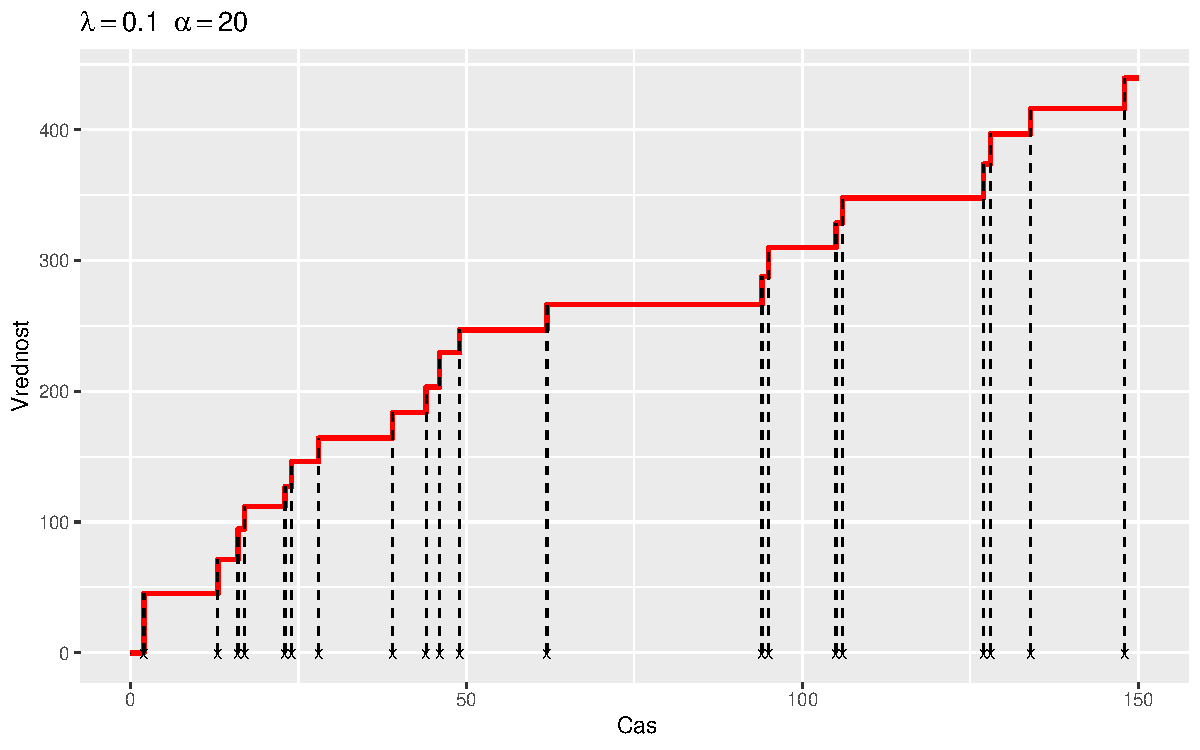
\includegraphics[width=\textwidth]{
            C:/Users/38651/OneDrive - Univerza v Ljubljani/Desktop/Diploma/Diplomski-seminar/GraphsAndPhotos/slika1.pdf
            }
        \caption{Primer trajektorije sestavljenega Poissonovega procesa}
        \label{fig:slika1}
    \end{figure}
    
    \noindent


    \begin{definicija}
        Naj bo $(\Omega, \mathcal{F}, \mathbb{P})$ verjetnostni prostor in naj bo $T\neq\emptyset$
        neprazna indeksna množica ter $(E, \Sigma)$ merljiv prostor. \textit{Slučajni proces}, 
        parametriziran s $T$, je družina slučajnih elementov $X_t : \Omega \to E$,
         ki so $(\mathcal{F}, \Sigma)$-merljivi za vsak $t \in T$.
        \label{def:slucProc}
    \end{definicija}

    \begin{opomba}
        V delu se bomo omejili na primer, ko $T$ predstavlja "cas, torej $T = [0, \infty)$ in da slu"cajne
        spremenljivke 
        zavzemajo vrednosti v realnih "stevilih, torej $(E, \Sigma) = (\R, \B_{\R})$, kjer $\B_\R$ 
        predstavlja Borelovo $\sigma-$algebro na $\R$.
        \label{op:Konvencije}
    \end{opomba}


    \begin{definicija}
        Za fiksen $\omega \in \Omega$ je preslikava 
        $[0, \infty) \rightarrow \mathbb{R}; \ t \mapsto X_t(\omega)$ 
        \textit{trajektorija} oziroma \textit{realizacija} slučajnega procesa $(X_t)_{t\geq0}$.
        Tako lahko slu"cajni proces gledamo kot predpis, ki vsakemu elementu vzor"cnega prostora 
        $\Omega$ priredi slu"cajno funkcijo
        $(X_t(\omega))_{t\geq0}: [0, \infty) \rightarrow \mathbb{R}$.
        \label{def:realizac}
    \end{definicija}

    \begin{definicija}
        Naj bo $(X_t)_{t\geq0}$ slu"cajni proces. Potem za $s < t$ definiramo
        \textit{prirastek procesa} $X_t - X_s$ na intervalu $[s, t]$. Proces $(X_t)_{t\geq0}$ ima 
        \textit{neodvisne prirastke}, če so za vsak nabor realnih "stevil
        $0 \leq t_1 < t_2 < \ldots < t_n < \infty$ prirastki
        $$
            X_{t_2} - X_{t_1}, \ X_{t_3} - X_{t_2}, \ \ldots, \ X_{t_n} - X_{t_{n-1}}
        $$
        med seboj neodvisni.
        \label{def:prirastek}
    \end{definicija}

    \begin{definicija}
        Naj bo $(X_t)_{t\geq0}$ slu"cajni proces. Potem pravimo, da ima proces
        \textit{stacionarne prirastke}, "ce za vsak $s < t$ in vsak $h > 0$ velja, 
        da ima $X_{t+h} - X_{s+h}$ enako porazdelitev kot $X_t - X_s$.
        \label{def:stacPrir}
    \end{definicija}

    \begin{definicija}
        Naj bosta $(X_t)_{t\geq0}$ in $(Y_t)_{t\geq0}$ slu"cajna procesa ne nujno definirana na istem 
        verjetnostnem prostoru. Pravimo, da sta $(X_t)_{t\geq0}$ in $(Y_t)_{t\geq0}$ \textit{neodvisna}, 
        "ce sta za vsak kon"cen nabor realnih "stevil $0 \leq t_1 < t_2 < \ldots < t_n < \infty$ slu"cajna 
        vektorja $(X_{t_1}, X_{t_2}, \ldots, X_{t_n})$ in $(Y_{t_1}, Y_{t_2}, \ldots, Y_{t_n})$ neodvisna.
        \label{def:neodvisnostSP}
    \end{definicija}

    \begin{definicija}
        Naj bo $\lambda > 0$. Slučajnemu procesu $(N_t)_{t\geq 0}$, definiranem na verjetnostnem 
        prostoru $(\Omega, \mathcal{F}, \mathbb{P})$ z vrednostmi v $\N_0$, pravimo 
        \textit{Poissonov proces} z intenzivnostjo $\lambda$, če zadošča naslednjim pogojem:
        \begin{enumerate}
            \item $N_0 = 0$ \ $\Prob$-skoraj gotovo.
            \item $(N_t)_{t\geq 0}$ ima neodvisne in stacionarne prirastke,
            \item Za $0 \leq s < t$ velja $ N_t - N_s \sim\Pois{\lambda(t - s)}$,
        \end{enumerate}
        \label{def:HPP}
    \end{definicija}
%\textcolor{red}{
%    \begin{opomba}
%        Vidimo, da v definiciji ne zahtevamo, da so skoki procesa le +1. To sledi iz...
%        \label{op:skoki}
%    \end{opomba}
%}

\section{Sestavljena Poissonova porazdelitev}

    \noindent
    Razdelek je prirejen po \cite{1}, \cite{2} in \cite{3}.

    Sestavljena poissonova porazdelitev je osnovni gradnik za sestavljeni Poissonov proces, ki ga obravnavamo 
    v naslednjem razdelku. Lastnosti, ki jih doka"zemo so direktno prenosljve na sam proces. Obravnavmo 
    porazdelitev in kako te pridemo, rodovne funkcije, zanimive rezultate v povezavi s 
    splo"snmi slu"cajnimi spremenljivkami in Panjerjevo rekurzivno shemo, ki jo prika"zemo na 
    prakti"cnem zgledu.

    \begin{definicija}
        Naj bo $N\sim \Pois{\lambda}$  za $\lambda >0$ in $X_1, X_2, \dots$ zaporedje neodvisnih (med seboj in $N$)
        enako porazdeljenih slučajnih spremenljivk. Potem pravimo, da ima slu"cajna spremenljivka
        \begin{equation*}
            S = \sum_{i=1}^NX_i
        \end{equation*}
        \textit{sestavljeno Poissonovo porazdelitev}. 
        \label{def:sestavljenaPoissonovaPorazdelitev}
    \end{definicija}

    \begin{opomba}
        V splo"snem lahko obravnavamo sestavljene porazdelitve kjer je $N$ poljubna slu"cajna spremenljivka,
        ki zavzema vrednosti v $\N_0$. Konkreten primer nas zanima zaradi njegove povezave s sestavljenim
        Poissonovim procesom. V nadaljevanju bomo uporabljali oznako
        \begin{equation*}
            S_0 = 0 \quad \text{in} \quad S_k = \sum_{i=1}^kX_i \quad \text{za} \ k\in\N, 
        \end{equation*}
        za pogojno porazdelitev $S\mid\{N = k\}$.
        \label{op:gneralCaseCOmpound}
    \end{opomba}

    \subsection{Porazdelitev}
    Z uporabo izreka o popolni verjetnosti s pogojevanjem na $N$ pridemo do formule za 
    porazdelitev $S$. Za $x \in \R$ velja 
    \begin{align*}
        F_{S}(x) = \Prob\bigl(S \leq x\bigr) 
        &= \sum_{k=0}^\infty \Prob\bigl(S \leq x \mid N = k\bigr)\Prob\bigl(N = k\bigr) \\
        &= \sum_{k=0}^\infty \Prob\bigl(S_k \leq x\bigr)\Prob\bigl(N = k\bigr) \\
        &= \sum_{k=0}^\infty F_{X_1}^{*k}(x) \frac{\lambda^k}{k!} e^{-\lambda},
    \end{align*}

    \noindent
    kjer je $F_{X_1}^{*k}(x)$ porazdelitev $k$-te konvolucije slu"cajne spremenljivke $X_1$.
    
    \begin{zgled}
        Poglejmo enega enostavnej"sih primerov, ko so $X_1, X_2, \dots$ porazdeljene kot
        \begin{equation*}
            X_1\sim\text{Exp}(a), \qquad \qquad f_{X_1}(x) = a e^{-a x}\mathbbm{1}_{(0, \infty)}(x),
        \end{equation*}
        s parametrom $a>0$. Vemo, da je $k$-ta 
        konvolucija $X_1$ porazdeljena kot \newline $\text{Gamma}(k, a)$ in ima gostoto
        \begin{equation*}
            f_{X_1 + \cdots + X_k}(x) = \frac{1}{\Gamma(k)}a^kx^{k-1}e^{-a x}\mathbbm{1}_{(0, \infty)}(x).
        \end{equation*}
        Za $s>0$ velja
        \begin{align*}
            F_{S}(s) 
            &= \sum_{k=0}^\infty \int_0^s\frac{1}{\Gamma(k)}a^kx^{k-1}e^{-ax}dx \ \frac{(\lambda )^k}{k!}e^{-\lambda }
            \qquad \qquad \text{Tonelli} \ (\ref{izr:TonellijevIzrek}) \\
            &= \int_0^s\underbrace{\sum_{k=0}^\infty \frac{1}{(k-1)!k!}(a\lambda)^kx^{k-1}e^{-(ax + \lambda)}}_{f_S(x)}dx.
        \end{align*}
        Vidimo, da "ze v primeru, ko poznamo eksplicitno formulo za $F^{*k}_{X_1}$, te"zko pridemo do 
        kakr"sne koli porazdelitve $S$ v kon"cni obliki. V praksi se zato poslu"zujemo numeri"cnega 
        ocenjevanja.
        \label{zgd:sestavljenaPoissonovaPorazdelitevGamma}
    \end{zgled}

    \subsection{Rodovne funkcije}

    \begin{trditev}
        Naj bo $N\sim \Pois{\lambda}$  za $\lambda >0$ in $X_1, X_2, \dots$ zaporedje neodvisnih (med seboj in $N$)
        enako porazdeljenih slučajnih spremenljivk s karakteristi"cno funkcijo $\varphi_{X_1}$. Potem ima za $u\in\R$
        karateristi"cna funckija $S = \sum_{i=1}^NX_i$ obliko
        \begin{equation*}
            \varphi_{S}(u) = e^{\lambda \left(\varphi_{X_1}(u) - 1\right)}.
        \end{equation*}
        \label{trd:MomentGener}
    \end{trditev}
    
    \begin{proof}
        Velja
        \begin{align}
            \varphi_{S}(u) 
                    &= \E\left[\exp\left[iuS\right]\right] \nonumber\\
                    &= \sum_{k=0}^{\infty}
                        \E\left[\exp\left[iuS \ \big| \ N=k\right]\right]\Prob\left(N = k\right) \nonumber \\ 
                    &= \sum_{k=0}^{\infty}
                        \E\left[\exp\left[iuS_k\right]\right]\Prob\left(N = k\right) \nonumber \\
                    &= \sum_{k=0}^{\infty}
                        \underbrace{\E\left[e^{iuX_1}\right]^k}_{\varphi_{X_1}(u)^k}\frac{\lambda^k}{k!}e^{-\lambda } \label{eq:MomentS}\\ 
                    &= e^{-\lambda } + e^{-\lambda }\sum_{k=1}^\infty\frac{\left(\varphi_{X_1}(u)\lambda \right)^k}{k!} \nonumber \\
                    &= e^{\lambda \left(\varphi_{X_1}(u) - 1\right)}. \nonumber
        \end{align}
    \end{proof}
    
    \begin{posledica}
        Rodovna in momentno rodovna funkcija $S=\sum_{i = 1}^{N}X_i$ imata obliko 
    \begin{equation*}
        G_{S}(u) = e^{\lambda \left(G_{X_1}(u) - 1\right)}, \qquad \text{in} \qquad
        M_{S}(u) = e^{\lambda \left(M_{X_1}(u) - 1\right)}.
    \end{equation*}
    \end{posledica}

    \begin{proof}
    V splo"snem velja, da je karakteristi"cna funkcija neke slu"cajne spremenljivke $X$ enaka
    njeni rodovni funckij izvrednoteni v $e^{iu}$, torej $\varphi_X(u) = G_X(e^{iu})$ in momentno rodovni 
    funkciji izvrednoteni v $iu$, torej $\varphi_X(u) = M_X(iu)$, "ce obstajata.
    \end{proof}

    V nadaljevanju bomo uporabljali predvsem karakteristi"cno funkcijo $\varphi_S$, saj je ta vedno definirana 
    za vsak $u\in\R$. Prav nam bo pri"sla tudi naslednja povezava med $\varphi_S$ in $G_S$. 

    \begin{lema}
        Karakteristi"cno funckijo $\varphi_S$ lahko izrazimo kot kompozitum rodovne funkcije $G_N$ in 
        karateristi"cne funkcije $\varphi_{X_1}$.

        \begin{align*}
            \varphi_{S}(u) = G_{N}\left(\varphi_{X_1}(u)\right).
        \end{align*}

        \label{lema:povezavaRodovneKarkateristicne}
    \end{lema}

    \begin{proof}
        Po ena"cbi (\ref{eq:MomentS}) iz trditve \ref{trd:MomentGener} za $u\in\R$ velja
        \begin{align*}
            \varphi_{S}(u) &= \sum_{k=0}^{\infty}
            \varphi_{X_1}(u)^n\frac{\lambda^k}{k!}e^{-\lambda} \\
            &= G_{N}\left(\varphi_{X_1}(u)\right).
        \end{align*}
    \end{proof}

    Vemo, da za neodvisne slu"cajne spremenljivke $X_1,  \dots, X_n$, ki so porazdeljene 
    kot $X_1\sim\Pois{\lambda_1}, \ \dots, \ X_n\sim\Pois{\lambda_n}$, 
    velja, da je njihova vsota $S = \sum_{i=1}^nX_i$ porazdeljena kot $S\sim\Pois{\lambda}$, kjer je
    $\lambda = \sum_{i=1}^n\lambda_i$. Izka"ze se, da ima sestavljena poissonova porazdelitev 
    podobno lastnost.

    \begin{definicija}
        Naj bo $(\lambda_k)_{k\in\N}$ zaporedje pozitivnih realnih "stevil za katerega velja 
        $\sum_{k=1}^\infty\lambda_k = 1$. Naj bodo $F_1, F_2, \dots$ porazdelitvene funckcije
        realnih slu"cajnih spremenljivk $X_1, X_2, \dots$ Potem 
        \begin{equation*}
            F = \sum_{k=1}^\infty\lambda_kF_k
        \end{equation*}
        pravimo \textit{me"sanica porazdelitev} $F_1, F_2, \dots$
    \end{definicija}
    \noindent
    O"citno je $F$ porazdelitvena funckija. "Ce definiramo 
    $$
    I \sim 
    \begin{pmatrix}
        1 & 2 & 3 & \dots \\
        \lambda_1 & \lambda_2 & \lambda_3 & \dots
    \end{pmatrix},
    $$
    vidimo, da je $F$ porazdelitev slu"cajne spremenljivke $X = \mathbbm{1}_{\{I = 1\}}X_1 + \cdots + \mathbbm{1}_{\{I = n\}}X_n$, 
    kar enostavno poka"zemo z uporabo zakona o popolni verjentnosti. Za poljuben $n\in\N$ in $x\in\R$ velja 
    \begin{align*}
        \Prob\left(X \leq x\right) 
        &= \sum_{k=1}^n\Prob\left(X \leq x \ \big| \ I = k\right)\Prob\left(I = k\right) \\
        &= \sum_{k=1}^n\Prob\left(X_k \leq x\right)\lambda_k \\
        &= \sum_{k=1}^nF_k(x)\lambda_k.
    \end{align*}
    Z enakim argumentom lahko poka"zemo, da je $\varphi_X(u) = \sum_{k=1}^\infty\lambda_k\varphi_{X_k}(u)$.


    \begin{trditev}
        Naj imajo neodvisne slu"cajne spremenljivke $S_1, \dots, S_n$ sestavljeno Poissonovo porazdelitev, torej 
        \begin{equation*}
            S_k = \sum_{i=1}^{N_k}X_i^{(k)} \quad \text{za} \ k=1, \dots, n,
        \end{equation*}
        kjer je $N_k\sim \Pois{\lambda_k}$ za $\lambda_k > 0$ in za vsak $k = 1, \dots, n$ je $(X_i^{(k)})_{i\in\N}$ 
        zaporedje neodvisnih enako porazdeljenih slu"cajnih spremenljivk. Potem velja   
        \begin{equation*}
            S = \sum_{k=1}^nS_k \sim \sum_{i=1}^{N}Y_i,
        \end{equation*}
        kjer je $N\sim\Pois{\lambda}$ s parametrom $\lambda = \sum_{k=1}^n\lambda_k$ in $(Y_i)_{i\in\N}$ zaporedje
        neodvisnih enako porazdeljenih slu"cajnih spremenljivk z me"sano porazdelitvijo
        \begin{equation*}
        F_{Y_1} = \sum_{k=1}^n\frac{\lambda_k}{\lambda}F_{X_1^{(k)}}.
        \end{equation*}
        \label{trd:vsotaCPDjeCPD}
    \end{trditev}

    \begin{proof}
        Karakteristi"cna funkcija $S_k$ ima obliko
        \begin{equation*}
            \varphi_{S_k}(u) = e^{\lambda_k\left(\varphi_{X_1^{(k)}}(u) - 1\right)}.
        \end{equation*}
        Ker so $S_1, \dots, S_n$ neodvisne, velja
        \begin{align*}
            \varphi_{S}(u) 
                &= \prod_{k=1}^n\varphi_{S_k}(u) \\
                &= \prod_{k=1}^n\exp\left[\lambda_k\left(\varphi_{X_1^{(k)}}(u) - 1\right)\right] \\
                &= \exp\left[\lambda\left(\sum_{k=1}^n \frac{\lambda_k}{\lambda} \varphi_{X_1^{(k)}}(u) - 1\right)\right].
        \end{align*}
        Po izreku o 
        enoli"cnosti (\ref{izr:enolicnost}) sledi $S\sim\sum_{i=1}^{N}Y_i$.
    \end{proof}

    Na podoben na"cin poka"zemo, kako se sestavljena Poissonova porazdelitev izra"za v primeru, ko so
    slu"cajne spremenljivke $X_i$ diskretno porazdeljene.

    \begin{trditev}
        Naj bo $N\sim \Pois{\lambda}$  za $\lambda >0$ in $X_1, X_2, \dots X_n$ neodvisne s.s. (neodvisne 
        med sabo in od $N$) enako porazdeljene kot
        $$ X_1\sim
        \begin{pmatrix}
            a_1 & a_2 & a_3  \dots & \\
            \tfrac{\lambda_1}{\lambda} & \tfrac{\lambda_2}{\lambda} & \tfrac{\lambda_3}{\lambda} \dots & 
        \end{pmatrix},
        $$
        kjer $(a_n)_{n\in\N}$ je poljubno zaporedje realnih "stevil in 
        $(\lambda_n)_{n\in\N}$ zaporedje pozitivnih realnih "stevil za katerega velja 
        ${\sum_{i=1}^\infty\lambda_i = \lambda}$.
        Potem velja 
        \begin{equation*}
            \sum_{j=1}^\infty a_jY_j \sim \sum_{j=1}^NX_j,
        \end{equation*}
        kjer so $Y_1,Y_2,  \dots$ neodvisne slu"cajne spremenljivke porazdeljene kot \\
        $\Pois{\lambda_1},\Pois{\lambda_2}, \dots$
        \label{trd:NXjeEnakoaY}
    \end{trditev}

    \begin{proof}
        S $\varphi_{Z_n}(u)$ ozna"cimo karakteristi"cno funkcijo slu"cajne spremenljivke 
        $Z_n := a_1Y_1 + a_2Y_2 + \dots + a_nY_n$ in s $\varphi_{Z}(u)$ karakteristi"cno funkcijo
        $Z:= \sum_{j=1}^{N}X_j$. Po neodvisnosti velja
        \begin{align*}
            \varphi_{Z_n}(u) 
                    &= \prod_{j=1}^{n}\varphi_{Y_j}(a_ju)\\
                    &= \prod_{j=1}^{n}\exp\left[\lambda_j\left(e^{a_j i u} - 1\right)\right] \\
                    &= \exp\left[\sum_{j=1}^{n}\lambda_j\left(e^{a_j i u} - 1\right)\right].
        \end{align*}

        \noindent
        Po lemi \ref{lema:povezavaRodovneKarkateristicne} velja
        \begin{align*}
            \varphi_{Z}(u) 
                    &= G_N\left(\varphi_{X_1}(u)\right) \\
                    &= \exp\left[\lambda\left(\varphi_{X_1}(u) - 1\right)\right] \\
                    & = \exp\left[\lambda\left(\sum_{j=1}^\infty\frac{\lambda_j}{\lambda}e^{a_jiu} - 1\right)\right]\\
                    &= \exp\left[\sum_{j=1}^{\infty}\lambda_j\left(e^{a_j i u} - 1\right)\right].
        \end{align*}

        \noindent 
        Vidimo, da za vsak $u\in\R$ \ $\varphi_{Z_n}(u)$ po to"ckah konvergira k $\varphi_{Z}(u)$, torej
        \begin{equation*}
            \varphi_{Z_n} \xrightarrow{n\to\infty}\varphi_Z
        \end{equation*}
        po Lévijevem izreku o kontinuiteti (\ref{izr:LevijevIzrek}) velja $Z_n \xrightarrow[n\to\infty]{d}Z$.
    \end{proof}

    Rezultat je zanimiv predvsem zato, ker nam za razliko od trditve \ref{trd:vsotaCPDjeCPD} pove, da 
    lahko slu"cajno vsoto izrazimo kot linearno kombinacijo oziroma vrsto Poissonovih slu"cajnih spremenljivk.

    \begin{opomba}
    Kaj pa v primeru, ko $X_i$ niso diskretno porazdeljene? Ali lahko
    trditev \ref{trd:NXjeEnakoaY} posplo"simo?
    Izka"ze se, da tudi v splo"snem dobimo konvergenco v porazdelitvi (nisem prepri"can "ce je to res). 
    Naj bo $F(x)$ porazdelitvena funkcija realno"stevilske slu"cajne spremenljivke $X_1$.
    Ideja je, da definiramo funkcijo $F_n(x) := F(\tfrac{k + 1}{n})$ na intervalu 
    $\bigl[\frac{k}{n}, \frac{k + 1}{n}\bigr)$ za $k\in\mathbb{Z}$.
        \begin{figure}[H]
            \begin{center}
            
                \begin{tikzpicture}
                    % coordinate system
                    \draw[->] (-0.75,0) -- (9,0) node[right] {$x$};
                    \draw[->] (2,0) -- (2,4.5) node[above] {$F, F_n$};
                    \draw (2, 3.4) -- (2, 3.4) node[left] {$1$};
                    \draw[dashed] (-0.75,3.2) -- (9,3.2);
                
                    % CDF of continuous random variable
                    \draw[cyan] (-0.75, 0.1) .. controls (0,0.2) and (2.2, 0.3) .. (2.8, 1.2);
                    \draw[->, cyan] (2.8, 1.2) .. controls (3.1, 1.7) and (3.6, 2) .. (5, 2.1);
                    \filldraw[cyan] (5, 2.5) circle (0.7pt);
                    \draw[cyan] (5, 2.5) .. controls (6, 2.8) and (7.5, 3) .. (9, 3.05) node[below] {$F(x)$};    
                
                    % CDF of F_n,   
                    \draw[->, red] (-0.75, 0.22) -- (0.25, 0.22);
                    \filldraw[red] (-0.75, 0.22) circle (0.7pt);
                    \draw[->, red] (0.25, 0.39) -- (1.25, 0.39);
                    \filldraw[red] (0.25, 0.39) circle (0.7pt);
                    \draw[->, red] (1.25, 0.74) -- (2.25, 0.74);
                    \filldraw[red] (1.25, 0.74) circle (0.7pt);
                    \draw[->, red] (2.25, 1.68) -- (3.25, 1.68);
                    \filldraw[red] (2.25, 1.68) circle (0.7pt);
                    \draw[->, red] (3.25, 2.01) -- (4.25, 2.01) node[above left]{$F_n(x)$};
                    \filldraw[red] (3.25, 2.01) circle (0.7pt);
                    \draw[->, red] (4.25, 2.58) -- (5.25, 2.58);
                    \filldraw[red] (4.25, 2.58) circle (0.7pt);
                    \draw[->, red] (5.25, 2.79) -- (6.25, 2.79);
                    \filldraw[red] (5.25, 2.79) circle (0.7pt);
                    \draw[->, red] (6.25, 2.94) -- (7.25, 2.94);
                    \filldraw[red] (6.25, 2.94) circle (0.7pt);
                    \draw[->, red] (7.25, 3.03) -- (8.25, 3.03);
                    \filldraw[red] (7.25, 3.03) circle (0.7pt);
                
                
                    %intervals of F_n
                
                \end{tikzpicture}
                \caption{Aproksimacija $F$ s $F_n$}
                \label{fig:slika2}
            \end{center}
        \end{figure}

    \noindent
    Kot je razvidno iz slike \ref{fig:slika2}, je $F_n(x)$ stopni"casta funkcija, ki aproksimira 
    porazdelitveno funkcijo $F(x)$. Vemo, da $F_n$ ustreza diskretni porazdelitvi

    $$ 
    \begin{pmatrix}
        & \dots & \frac{k}{n} & \frac{k + 1}{n} & \frac{k+2}{n} & \dots & \\
        & \dots & F(\frac{k}{n}) - F(\frac{k-1}{n}) & F(\frac{k+1}{n}) - F(\frac{k}{n}) & F(\frac{k+2}{n}) - F(\frac{k+1}{n}) & \dots & 
    \end{pmatrix}.
    $$
    Izka"ze se, da $F_n \xrightarrow{n\to\infty}F$ povsod kjer je $F$ zvezna, ampak
    dokaz presega obseg tega dela. Interesirani bralec ga lahko najde v \cite{4} (moram dobiti dejansko referenco).
    \label{op:aproksimacijaZDiskretno}
    \end{opomba}





    \subsection{Panjerjeva rekurzivna shema}
    Poglejmo si popularno metodo za ra"cunaje sestavljene Poissonove porazdelitve v praksi. Kot
    smo videli v zgledu \ref{zgd:sestavljenaPoissonovaPorazdelitevGamma}, je ra"cunanje eksplicitne 
    porazdelitve $S$ v kon"cni obliki v splo"snem nemogo"ce. Izka"ze pa se, da jo je v posebnih primerih vselej mogo"ce
    rekurzivno izraziti in ustrezno posplo"siti na "sir"si razred porazdelitev.

    \begin{trditev}(Panjer)
        Naj bo $N$ diskretna slu"cajna spremenljivka, za katero velja 
        \begin{equation*}
            \Prob(N = n) = \left(a + \frac{b}{n}\right)\Prob\left(N = n-1\right) \quad \text{za} \ n\in\N \ \text{in} \ a, b \in \R.
        \end{equation*}
        Naj bo $X_1, X_2, \dots$ zaporedje neodvisnih in enako porazdeljenih slu"cajnih spremenljivk, ki 
        zavzemajo vrednosti v $\N_0$. Potem za $S = \sum_{i=1}^NX_i$ velja
        \begin{equation*}
        \Prob\left(S = 0\right) = 
        \begin{cases}
            \Prob\left(N = 0\right), & \text{če} \ \Prob(X_1 = 0) = 0, \\  
            \E\left[\Prob\left(X_1 = 0\right)^N\right], & \text{sicer}, 
        \end{cases}
        \end{equation*}
        in za $n\in\N$ velja
        \begin{equation}
            \Prob\left(S = n\right) = \frac{1}{1 - a\Prob\left(X_1 = 0\right)}\sum_{k = 1}^n\left(a + \frac{bk}{n}\right)\Prob\left(X_1 = k\right)\Prob\left(S = n - k\right).
            \label{eq:PanjerRecursionScheme}
        \end{equation}
        \label{tdr:PanjerRecursionScheme}
    \end{trditev}

    \begin{proof}
        Prvo se osredoto"cimo na primer $n = 0$. Velja
        \begin{align*}
            \Prob\left(S = 0\right)     
                = \Prob\left(N = 0\right) + \Prob\left(S = 0, N > 0\right).
        \end{align*}
        "Ce velja $\Prob(X_1 = 0) = 0$, je enakost o"citna. "Ce 
        velja $\Prob(X_1 = 0) > 0$, po zakonu za popolno pri"cakovano vrednsot ra"cunamo
        \begin{align*}
            \Prob\left(S = 0\right) 
                &= \Prob\left(N = 0\right) + \sum_{k = 1}^\infty\Prob\left(S = 0, N > 0 \mid N = k\right)\Prob\left(N = k\right) \\
                &= \Prob\left(N = 0\right) + \sum_{k = 1}^\infty\Prob\left(S_k = 0\right)\Prob\left(N = k\right) \\
                &= \Prob\left(N = 0\right) + \sum_{k = 1}^\infty\Prob\left(X_1 = 0\right)^k\Prob\left(N = k\right) \\
                &= \E\left[\Prob\left(X_1 = 0\right)^N\right].
        \end{align*}
        Za $n\in\N$ velja
        \begin{align}
            \Prob\left(S = n\right) 
                &= \sum_{k = 1}^\infty\Prob\left(S_k = n\right)\Prob\left(N = k\right) \nonumber \\
                &= \sum_{k = 1}^\infty\Prob\left(S_k = n\right)\left(a + \frac{b}{k}\right)\Prob\left(N = k - 1\right). \label{eq:PanjerRecursionSchemeProof}
        \end{align}
        "Ce sedaj upo"stevamo, da so $X_i$ neodvisne in enako porazdeljene, opazimo, da velja
        \begin{equation*}
            1 = \E\left[\frac{S_k}{S_k}\ \bigg| \ S_k\right] = \sum_{i = 1}^k\E\left[\frac{X_i}{S_k}\ \big| \ S_k\right] = k\E\left[\frac{X_1}{S_k}\ \big| \ S_k\right],
        \end{equation*}
        torej je 
        \begin{equation*}
            \E\left[\frac{X_1}{S_k} \ \bigg| \ S_k\right] = \frac{1}{k}
        \end{equation*}
        in posledi"cno 
        \begin{equation}
            \E\left[a + \frac{bX_1}{n}\ \bigg| \  S_k = n\right] = a + \frac{b}{k}.
            \label{eq:PanjerRecursionSchemeProof2}
        \end{equation}         
        Nadaljno velja  
        \begin{align}   
            & \E\left[a + \frac{bX_1}{n}\ \bigg| \  S_k = n\right] \nonumber \\
            &= \sum_{i = 0}^n\left(a + \frac{bi}{n}\right)\Prob\left(X_1 = i\mid S_k = n\right) \nonumber \\
            &= \sum_{i = 0}^n\left(a + \frac{bi}{n}\right)\frac{\Prob\left(X_1 = i, S_k - X_1 = n - i\right)}{\Prob\left(S_k = n\right)} \nonumber \\
            &= \sum_{i = 0}^n\left(a + \frac{bi}{n}\right)\frac{\Prob\left(X_1 = i\right)\Prob\left(S_{k- 1} = n - i\right)}{\Prob\left(S_k = n\right)} \label{eq:PanjerRecursionSchemeProof3} 
        \end{align}
        "Ce sedaj vstavimo enakost (\ref{eq:PanjerRecursionSchemeProof2}) v (\ref{eq:PanjerRecursionSchemeProof}) 
        in upo"stevamo (\ref{eq:PanjerRecursionSchemeProof3}), dobimo
        \begin{align*}
            \Prob\left(S = n\right) 
                = \sum_{k = 1}^\infty\sum_{i = 0}^n \left(a + \frac{bi}{n}\right)\Prob\left(X_1 = i\right)\Prob\left(S_{k - 1} = n - i\right)\Prob\left(N = k - 1\right).
        \end{align*}
        Po Tonellijevem izreku (\ref{izr:TonellijevIzrek}) lahko zamenjamo vrstni red integracije, da dobimo
        \begin{align*}
            \Prob\left(S = n\right) 
                &= \sum_{i = 0}^n\left(a + \frac{b}{n}\right)\Prob\left(X_1 = i\right)\sum_{k = 1}^\infty\Prob\left(S_{k - 1} = n - i\right)\Prob\left(N = k - 1\right)\\
                &= \sum_{i = 0}^n\left(a + \frac{b}{n}\right)\Prob\left(X_1 = i\right)\Prob\left(S = n - i\right).
        \end{align*}
        Izpostavimo prvi "clen vsote in izraz preoblikujemo.
        \begin{align*}
            \Prob\left(S = n\right) 
                &= a\Prob\left(X_1 = 0\right)\Prob\left(S = n\right) + \sum_{i = 1}^n\left(a + \frac{b}{n}\right)\Prob\left(X_1 = i\right)\Prob\left(S = n - i\right), \\
            \Prob\left(S = n\right)
                &= \frac{1}{1 - a\Prob\left(X_1 = 0\right)}\sum_{i = 1}^n\left(a + \frac{b}{n}\right)\Prob\left(X_1 = i\right)\Prob\left(S = n - i\right).
        \end{align*}
        S tem je trditev dokazana.
    \end{proof}

    \begin{opomba}
        Izka"ze se, da le $3$ porazdelitve 
        ustrezajo pogojem iz trditve \ref{tdr:PanjerRecursionScheme}. Te so $\Pois{\lambda}$, $\text{Bin}(p)$ in
        $\text{NegBin}(r, p)$. Pravimo jim \textit{porazdelitve Panjerjevega razreda}. V primeru $N\sim\Pois{\lambda}$ za $n\in\N$, $a = 0$ in $b = \lambda$ velja $\Prob\left(N = n\right) = \frac{\lambda^n}{n!}e^{-\lambda} = 
        \left(0 + \frac{\lambda}{n}\right)\Prob\left(N = n - 1\right)$. Tudi v ostalih primerih se izka"ze, da je $a < 1$, tako da je 
        ena"cba (\ref{eq:PanjerRecursionScheme}) res dobro definirana.
    \end{opomba}

    \begin{opomba}
        Zahtevo, da $X_i$ zavzemajo vrednosti v $\N_0$ lahko sprostimo. V resnici 
        lahko zahtevamo le, da $X_i$ zavzemajo vrednosti v $h\N_0$ za nek $h>0$. V tem primeru 
        zapi"semo $S = h\sum_{i=1}^N\frac{X_i}{h}$ in tako rekurzivna zveza velja za $\frac{S}{h}$. 
        Tako lahko kot v ideji opombe \ref{op:aproksimacijaZDiskretno} aproksimiramo splo"sne slu"cajne 
        spremenljivke, ki zavzemajo vrednsoti v $[0, \infty)$, poljubno natan"cno.
    \end{opomba}  

    \begin{zgled}(Nadaljevanje zgleda \ref{zgd:sestavljenaPoissonovaPorazdelitevGamma}) Recimo, da imamo
        konkretni porazdeltivi $N\sim\Pois{9}$ in $X_i\sim\text{Exp}(\frac{1}{\pi})$. Podobno kot v opombi
        \ref{op:aproksimacijaZDiskretno} s stopni"castima funkcijama
        $F^u_h$ in $F_h^l$ aproksimiramo porazdelitveno funkcijo $F_{X_1}$ za razli"cne vrednosti $h \in \{1, \ 0,1\}$.
        Za vsak $n\in\N$ velja $F^u_h(x) = F_{X_1}((n+1)h)$ za $x\in\bigl[nh, (n+1)h\bigr)$ in 
        $F^l_h(x) = F_{X_1}(nh)$ za $x\in\bigl[nh, (n+1)h\bigr)$.
        S Panjerjevo rekurzivno shemo izra"cunamo pribli"zke porazdelitve $S$ na intervalu $[0, 60]$.
        Rezulate prika"zemo na sliki \ref{fig:slika7}. 
 
        \begin{figure}[h!]
            \begin{center}
                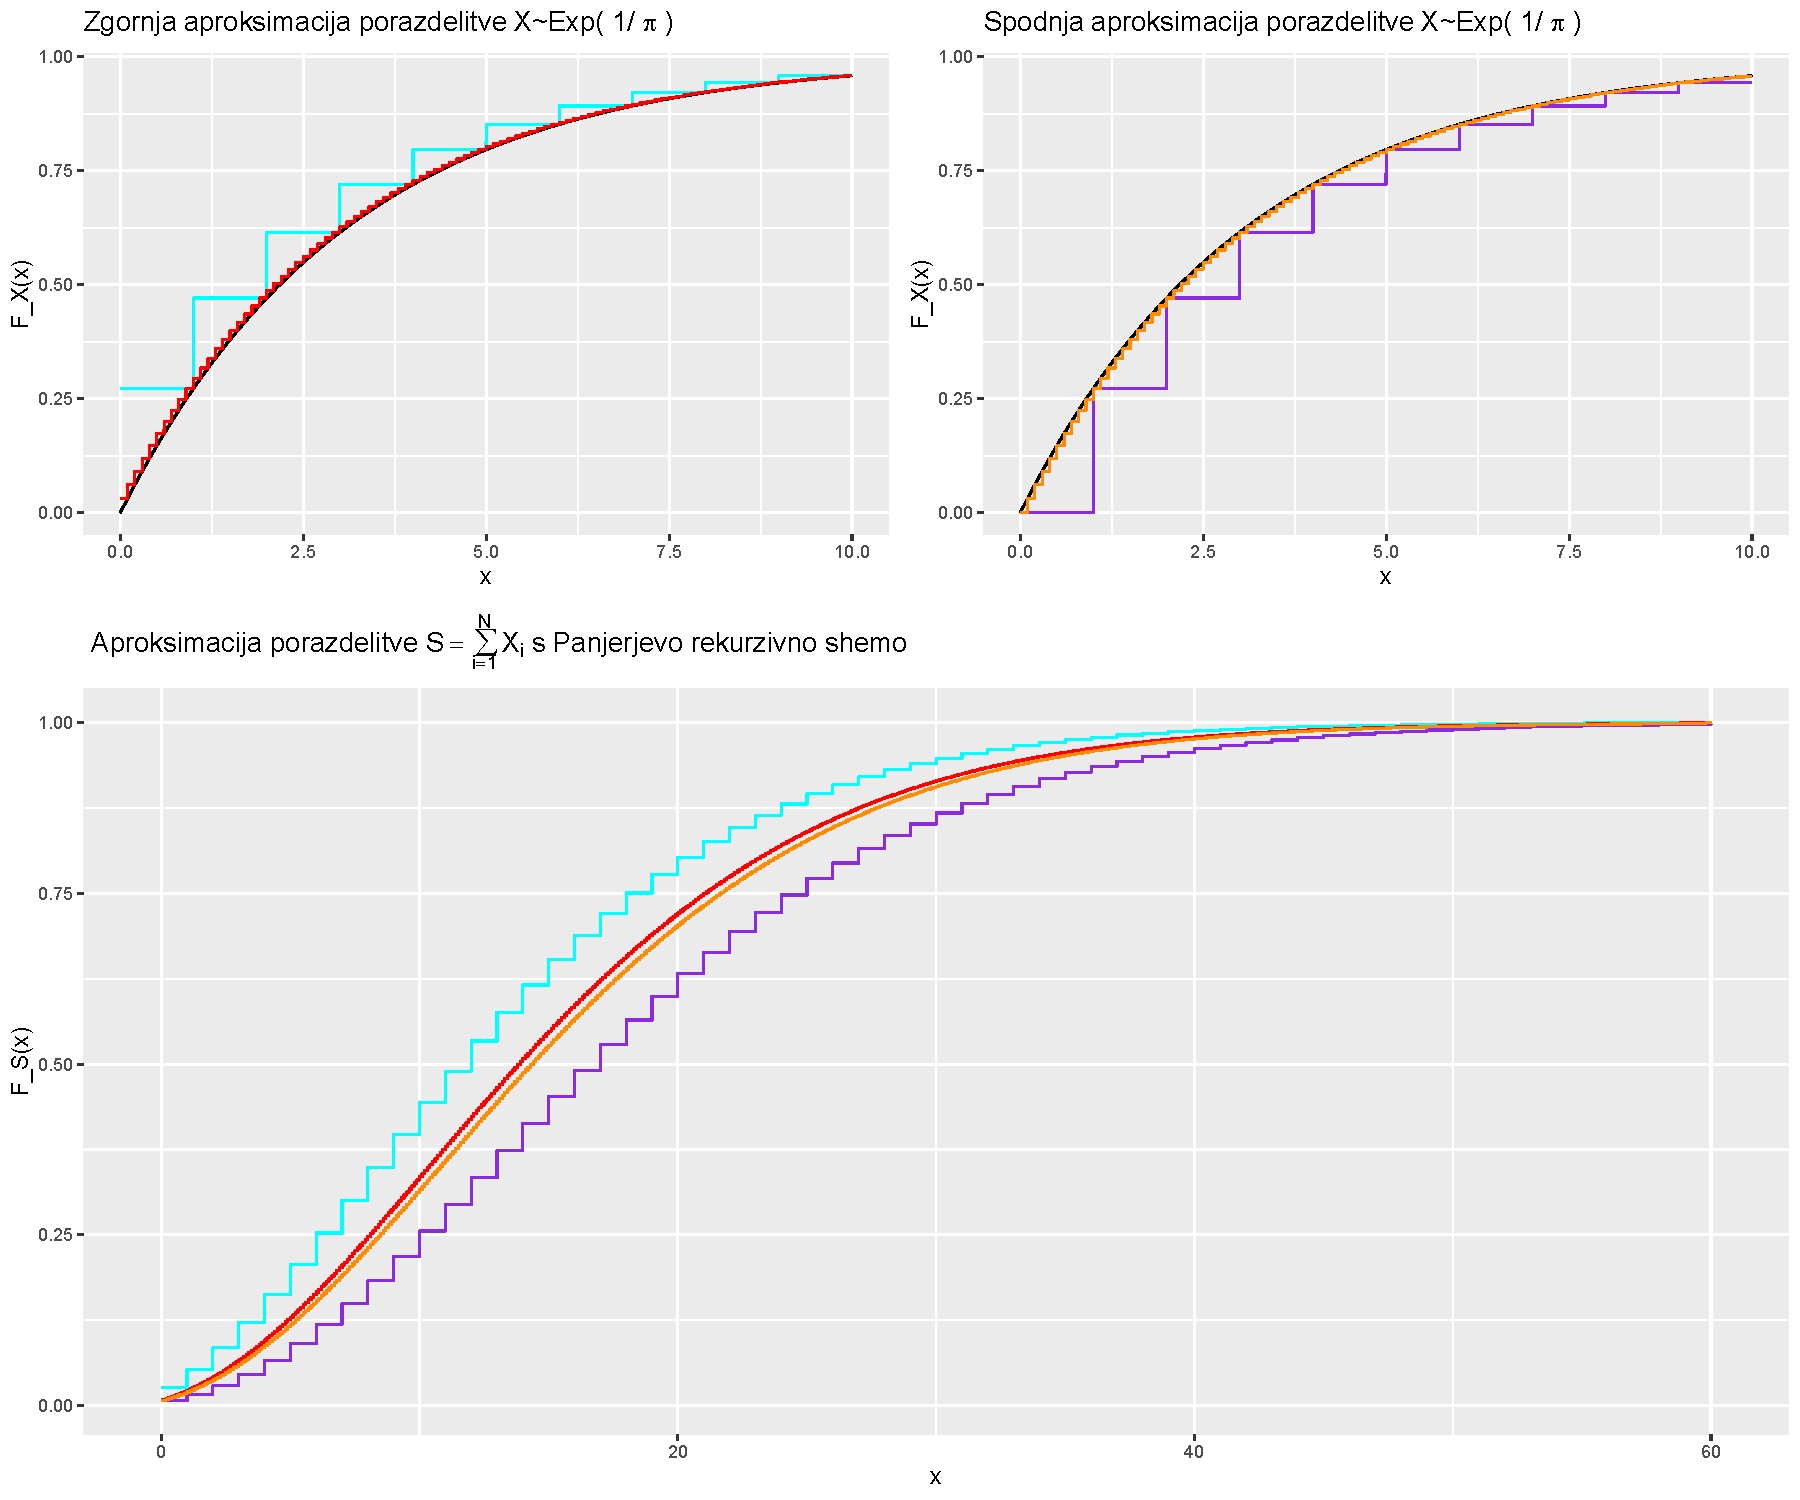
\includegraphics[width=\textwidth]{
                    C:/Users/38651/OneDrive - Univerza v Ljubljani/Desktop/Diploma/Diplomski-seminar/GraphsAndPhotos/slika7.pdf
                }
                \caption{Aproksimacija porazdelitve $S$ s Panjerjevo rekurzivno shemo.}
                \label{fig:slika7}
            \end{center}
        \end{figure}
        
        \label{zgd:PanjerExp}  
    \end{zgled}
 
    Vidimo, da "ze za $h = 0,1$ dobimo zelo natan"cno aproksimacijo porazdelitve. Danes 
    Panjerjeva metoda predstavlja alternativo Monte Carlo metodam. Njena glavna prednost 
    je, da z manj"sanjem koraka $h$ dose"zemo poljubno natan"cno to"cno aproksimacijo neke porazdelitve. 
    Monte Carlo metode so bolj splo"sne, saj temeljijo zgolj na ponavljanju simulacij in se lahko uporabljajo za modeliranje bolj zapletenih 
    porazdelitev, ki ne zadovoljujejo pogojev trditve \ref{tdr:PanjerRecursionScheme}.

\pagebreak
\section{Sestavljeni Poissonov proces}

    \noindent
    Razdelek je prirejen po \cite{1}, \cite{2}, in \cite{3}.

    Poka"zemo, da ima sestavljeni Poissonov proces neodvisne in stancionarne prirastke. Markiranje, pokazemo 
    da spada v sirsi razred slucajnih procesov t.i.\ Levijevih procesov.


    \begin{definicija}
        Naj bo $(N_t)_{t\geq0}$ Poissonov proces z intenzivnostjo $\lambda$. 
        Naj bo $(X_i)_{i\geq1}$ zaporedje neodvisnih (med sabo in $(N_t)_{t\geq0}$) in enako 
        porazdeljenih slučajnih spremenljivk z vrednostmi v $\mathbb{R}$. Potem je 
        \textit{sestavljeni Poissonov proces} $(S_t)_{t\geq0}$ definiran kot dru"zina
        slu"cajnih spremenljivk
        $$
            S_t = \sum_{i=1}^{N_t} X_i, \quad t\geq0.
        $$
        \label{def:CPP}
    \end{definicija}

    \begin{opomba}
        Vidimo, da je sestavljeni Poissonov proces naravna posplo"sitev homogenega Poissonovega procesa, saj "ce za
        $X_i$ vzamemo konstantno funkcijo $X_i = 1$ za vsak $i$, je to ravno $HPP(\lambda)$. Bolj v splo"snem, "ce je 
        $X_i = \alpha$ deterministi"cna funkcija, potem velja $S_t = \alpha N_t$.
        \label{op:CPPHPPPovezava}
    \end{opomba}

    V nadaljevanju bomo homogen Poissonov proces z intenzivnostjo $\lambda >0$ ozna"cevali s $HPP(\lambda)$ 
    ali naborom slu"cajnih spremenljivk $(N_t)_{t\geq0}$ (angl. Homogeneous Poisson Process), 
    sestavljeni Poissonov proces pa s $CPP$ ali naborom slu"cajnih spremenljivk $(S_t)_{t\geq0}$ 
    (angl. Compound Poisson Process), kjer bo vsota sledila $HPP(\lambda)$. 

    \subsection{Osnovne lastnosti}
    
        Kot smo nakazali v uvodu dela, nas pri "studiranju slu"cajnih procesov najprej zanimajo osnovne 
        lastnosti s katerimi je la"zje delati kot z ne"stevnim naborom slu"cajnih spremenljivk in s pomo"cjo 
        katerih lahko poka"zemo globje rezultate o procesu. 

        \begin{trditev}
            Naj bo $(X_t)_{t\geq0}$ slu"cajni proces na $(\Omega, \F, \mathbb{P})$ in naj velja $X_0 = 0$ s.g.
            Potem ima $(X_t)_{t\geq0}$
            neodvisne prirastke natanko tedaj, ko je za vsak nabor "stevil 
            $0 \leq t_1 < \ldots < t_n < t_{n+1} <\infty$ prirastek $X_{t_{n+1}} - X_{t_n}$ neodvisen od
            slu"cajnega vektorja $(X_{t_1}, \dots, X_{t_n})$.
            \label{trd:ekvivKarakterizacija}
        \end{trditev}

        \begin{proof}
            $(\Leftarrow):$ Recimo, da je za vsak $n\in\N$ in poljuben nabor "stevil $0 \leq t_1 < \ldots < t_n < t_{n+1} <\infty$ 
            prirastek $X_{t_{n+1}} - X_{t_n}$ neodvisen od slu"cajnega vektorja $(X_{t_1}, \dots, X_{t_n})$.
            Potem je $X_{t_{n+1}} - X_{t_n}$ neodvisen tudi od $h(X_{t_1}, \dots, X_{t_n})$ za poljubno merljivo funkcijo $h:\R^n\to \R^n$.
            O"citno je $(X_{t_1}, \dots, X_{t_n}) \mapsto (X_{t_2} - X_{t_1}, \dots, X_{t_{n}} - X_{t_{n-1}})$ taka funkcija,
            torej je $X_{t_{n+1}} - X_{t_n}$ neodvisen od $(X_{t_2} - X_{t_1}, \dots, X_{t_{n}} - X_{t_{n-1}})$. Ker 
            to velja za poljuben $n$ in poljubne $t_i$, sledi, da ima $(X_t)$ neodvisne prirastke. \newline
            $(\Rightarrow):$  Recimo, da ima $(X_t)_{t\geq0}$ neodvisne prirastke. Ker velja $X_0 = 0$ s.g., vemo, da 
            je za poljuben $n\in\N$ in poljuben nabor "stevil $0 \leq t_1 < \ldots < t_n < t_{n+1} <\infty$
            prirastek $X_{t_{n+1}} - X_{t_n}$ neodvisen od $(X_0, X_{t_1} - X_0, \dots, X_{t_n} - X_{t_{n-1}})$ in posledi"cno neodvisen od
            $h(X_0, X_{t_1} - X_0, \dots, X_{t_n} - X_{t_{n-1}})$ za poljubno merljivo funkcijo $h:\R^{n+1}\to \R^{n+1}$, ki 
            jo definiramo na slede"c na"cin:
            \begin{align*}
                h(x_0, x_1, \dots, x_n) &= (h_0, h_1, \dots, h_n),\\
                                    h_0 &= x_0, \\
                                    h_1 &= x_0 + x_1, \\
                                    &\mathrel{\makebox[\widthof{=}]{\vdots}} \\
                                    h_n &= x_0 + x_1 + \cdots + x_n.
            \end{align*}
            Tako velja $h(X_0, X_{t_1} - X_0, \dots, X_{t_n} - X_{t_{n-1}}) = (X_0, X_{t_1}, \dots, X_{t_n})$ in s tem je trditev dokazana.

        \end{proof}

        \begin{trditev}
            $CPP$ ima neodvisne in stacionarne prirastke.
            \label{trd:neodvPrirCPP}
        \end{trditev}

        \begin{proof}
            Za nabor realnih "stevil $0 \leq t_1 < \ldots < t_{n+1}  < \infty$ lahko slu"cajne
            spremeljivke $S_{t_i} - S_{t_{i-1}}$ zapi"semo kot
            \begin{align*}
                S_{t_i} - S_{t_{i-1}} &= X_{N_{t_{i - 1} + 1}} + \cdots + X_{N_{t_i}} 
            \end{align*}
            Neodvisnost prirastkov sledi po neodvisnosti $X_i$ od $X_j$ za $i\neq j$ in $N_t$. 
            Naj bo $h > 0$ in $s < t$. Potem velja
            \begin{align*}
                S_{t+h} - S_{s+h} &= \sum_{j=N_{s+h}+1}^{N_{t+h}} X_j \\
            \end{align*}
            Vsota ima $N_{t+h} - N_{s+h}$ členov. Ker za $HPP$ velja 
            $N_{t+h} - N_{s+h} \sim N_t - N_s$, je 
            \begin{align*}
                \sum_{j=N_{s+h}+1}^{N_{t+h}} X_j \sim \sum_{j=N_{s}+1}^{N_{t}} X_j = S_t - S_s.
            \end{align*}
        \end{proof}

        \begin{opomba}
            Podobno kot v opombi \ref{op:gneralCaseCOmpound} za $k\in\N_0$ pogojno porazdelitev $S_t \mid \{N_t = k\}$ 
            ozna"cimo s
            \begin{equation*}
                S_{t, 0} = 0 \quad \text{in} \quad S_{t, k} = \sum_{i=1}^kX_i \quad \text{za} \ k\in\N.
            \end{equation*}
        \end{opomba}

        \begin{trditev}
            Naj bo $(S_t)_{t\geq 0}$ $CPP$ in naj bosta $\mu = \E\left[X_i\right] < \infty$ 
            pri"cakovana vrednost in $\sigma^2= \Var{X_i} <\infty$ varianca
            slu"cajnih spremenljivk $X_i$. Potem sta za $t\geq0$ pri"cakovana vrednost in 
            varianca $S_t$ enaki 
            \begin{equation*}
                \E\left[S_t\right] = \mu\lambda t \qquad \text{in} \qquad \Var{S_t} = \lambda t\left(\sigma^2 + \mu^2\right).
            \end{equation*}
            \label{trd:PricVarCPP}
        \end{trditev}

        \begin{proof}

            Za $t\geq0$ $S_t$ pogojno na $N_t = k$ velja
            \begin{align*}
            \E\left[S_t\mid N_t = k\right] = \E\left[Y_k\right] = k\mu \qquad \text{in} \qquad
            \Var{S_t\mid N_t = k} = \Var{Y_k} = k\sigma^2.
            \end{align*}
            Po formuli za popolno pri"cakovano vrednost velja 
            $\E\left[S_t\right] = \E\left[\E\left[S_t\mid N_t\right]\right]$. Torej

            \begin{align*}
                \E\left[S_t\right] = \E\left[\E\left[S_t\mid N_t\right]\right] = \E\left[\mu N_t\right] = \mu\lambda t.
            \end{align*}

            \noindent
            Prek formule $\Var{S_t} = \E\left[\Var{S_t\mid N_t}\right] + \Var{\E\left[S_t\mid N_t\right]}$ ra"cunamo 

            \begin{equation*}
                \E\left[\Var{S_t\mid N_t}\right] = \E\left[\Var{X_i}N_t\right] = \sigma^2\lambda t
            \end{equation*}
            in 
            \begin{equation*}
                \Var{\E\left[S_t\mid N_t\right]} = \Var{\E\left[X_i\right]N_t} = \mu^2\lambda t.
            \end{equation*}
            "Ce ena"cbi sestejemo, dobimo $\Var{S_t} = \lambda t\left(\sigma^2 + \mu^2\right)$.
        \end{proof}
    
    \begin{zgled}
        Poglejmo si primer ko je zaporedje $(X_i)_{i\in\N}$ porazdeljeno kot $X_1\sim N(2, 42)$ 
        Tedaj za $t\geq 0 $ velja $\E\left[S_t\right] = 2t$ in 
        $\Var{S_t} = t(2^2 + 42^2) = 1768t$ ter $\sigma_{S_t} = \sqrt{1768t}$. Simuliramo 10 realizacij CPP do "casa $T=1000$, 
        ki jih prika"zemo na sliki \ref{fig:slika6} skupaj s funkcijama $t \mapsto \E\left[S_t\right]$ in $t \mapsto \E\left[S_t\right] \pm 3\sigma_{S_t}$. 
        \begin{figure}[H]
            \centering
            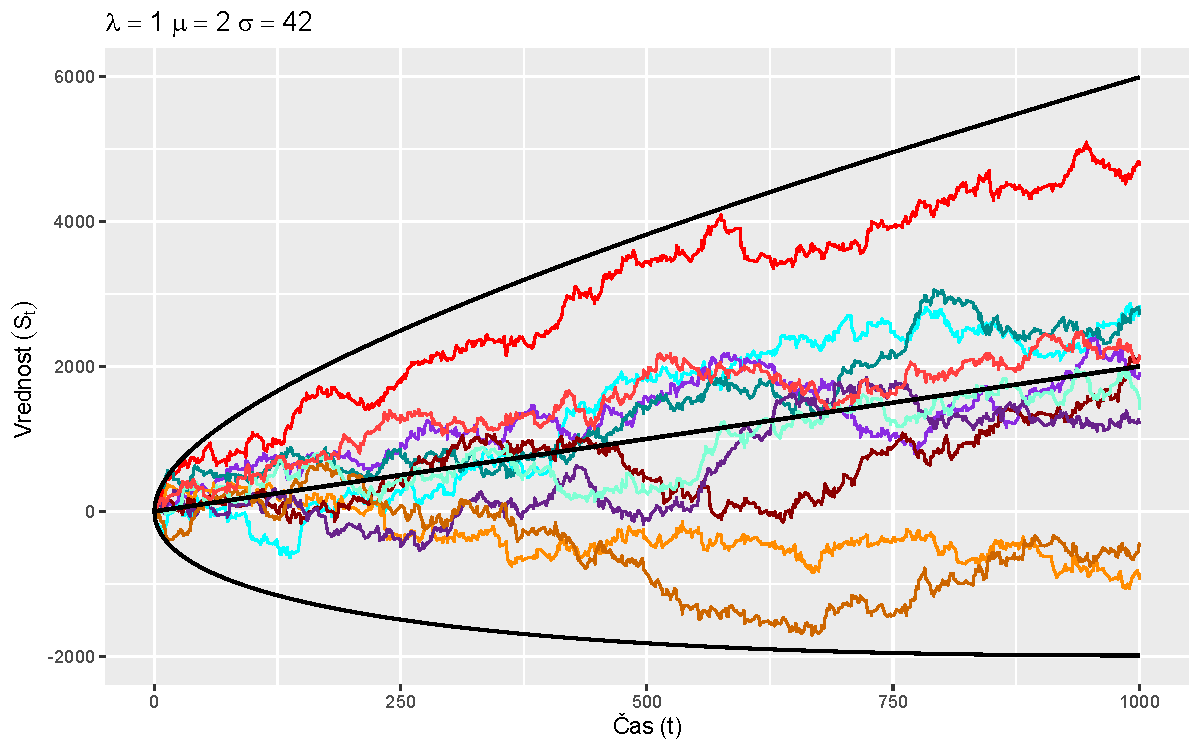
\includegraphics[width=\textwidth]{
                C:/Users/38651/OneDrive - Univerza v Ljubljani/Desktop/Diploma/Diplomski-seminar/GraphsAndPhotos/slika6.pdf
                }
            \caption{Trajektorije CPP s funckijama $t \mapsto \E\left[S_t\right]$ in $t \mapsto \E\left[S_t\right] \pm 3\sigma_{S_t}$}
            \label{fig:slika6}
        \end{figure}

    \end{zgled}
    %Poka"zimo, da je $CPP$ v resnici porazdeljen, kot limita linearne 
    %kombinacije neodvisnih Poissonovih slu"cajnih spremenljivk. 
    
    %\noindent
    %"Ce sedaj po"sljemo $n \to \infty$, dobimo
    %\begin{align}
    %    \varphi_{Z}(u) := \lim_{n\to\infty}\varphi_{Z_n}(u) = e^{\sum_{j=1}^{\infty}\lambda_j\left(e^{a_j i u} - 1\right)}.
    %    \label{eq:karFunkcVrste}
    %\end{align}
%
    %\noindent
    %Kot smo izpeljali zgoraj je karakteristi"cna funkcija $CPP$ podana s predpisom
%
    %\begin{align*}
    %    \varphi_{S_t}(u) = e^{\lambda t\left(\varphi_X(u) - 1\right)}, 
    %\end{align*}
%
    %\noindent
    %kar lahko zapi"semo kot 
%
    %\begin{align*}
    %    \varphi_{S_t}(u) = e^{\lambda t\int_{\R}\left(e^{i u z} - 1\right) \mu(dz)},
    %\end{align*}
%
    %\noindent
    %kjer je $\mu := X*\Prob$ potisk mere naprej po s.s.\ $X$. Prav tako lahko (\ref{eq:karFunkcVrste}) zapi"semo
    %kot 
%
    %\begin{align*}
    %    \varphi_{Z}(u) = e^{\int_{\R}\left(e^{i u x} - 1\right)\nu(dx)},
    %\end{align*}
%
    %\noindent
    %Za neko ustrezno mero $\nu$. Vidimo, da ko po"sljemo $n\to \infty$, za ustrezen izbor 
    %$a_1, a_2, \dots$ in $\lambda_1, \lambda_2, \dots$ karakteristi"cna funkcija 
    %vrste $Z_n$ konvergira h karakteristi"cni funkciji $S_t$. Torej po Lévijevem izreku o zveznosti 
    %sledi, da je $S_t$ enako porazdeljena kot $Z = \sum_{i=1}^{\infty}\alpha_iY_i$.
%

%    \subsection{Martingali}
%
%        \begin{definicija}
%            Slu"cajni proces $X_t$ prilagojen glede na filtracijo (\ref{def:filtracija}) $(\F_t)_{t\geq0}$
%            martingal, "ce velja 
%            $$
%                \E\left[X_t\mid\F_s\right] = X_s
%            $$
%            za vsak $0\leq s \leq t$.
%            \label{def:martingal}
%        \end{definicija}
%
%        \begin{trditev}
%            Naj bo $(S_t)_{t\geq0}$ $CPP$ z intenzivnostjo $\lambda>0$ in naj bodo $X_i$ neodvisne
%            in enako porazdeljene slu"cajne spremenljivke z $\E\left[X_i\right] = \mu$ za vsak $i$.
%            Potem je $S_t$ martingal natanko tedaj, ko je $\mu = 0$.
%            \label{trd:CPPnimartingal}
%        \end{trditev}
%
%        \begin{proof}
%            Naj bo $0\leq s\leq t$. Potem velja
%            \begin{align*}
%                \E\left[S_t\mid\F_s\right] 
%                        &= \E\left[S_t - S_s + S_s\mid \F_s\right] \\
%                        &= \E\left[S_t - S_s\right] + \E\left[S_s\mid \F_s\right] \\
%                        &= \mu\lambda(t-s) + S_s
%            \end{align*}
%           Enakost $\mu\lambda(t-s) + S_s = S_s$ velja $\iff$ $\mu\lambda(t-s) = 0 \iff \mu = 0$.
%        \end{proof}
%
%        \begin{opomba}
%            Seveda, "ce velja $\mu \geq 0$, potem je $S_t$ submartingal, "ce pa $\mu \leq 0$, je
%            $S_t$ supermartingal.
%        \end{opomba}
%
%        \begin{posledica}
%            Za poljuben $\mu \in \R$ je proces 
%            $$
%                S_t - \mu\lambda t
%            $$
%            martingal. 
%            \label{trd:CPPpostanemartingal}
%        \end{posledica}
%
%        \begin{proof}
%            Naj bosta $0 \leq s < t$. Velja
%            \begin{align*}
%                \E\left[S_t - \mu\lambda t\mid\F_s\right] 
%                        &= \E\left[S_t - S_s\right] + S_s - \mu\lambda t\\
%                        &= \mu\lambda(t-s) + S_s - \mu\lambda t\\
%                        &= S_s - \mu\lambda s.
%            \end{align*}
%        \end{proof}
%
%    \subsection{"Casi ustavljanja in lastnosti Markova}
%        \begin{definicija}
%            Naj bo $(\Omega, \mathcal{F}, \mathbb{P}, (\mathcal{F}_t)_{t\geq0})$ filtriran verjetnostni 
%            prostor. Slu"cajna spremenljivka 
%            $$
%            \tau : \Omega \to [0, \infty]
%            $$ 
%            je \textit{"cas ustavljanja} glede na filtracijo $(\mathcal{F}_t)_{t\geq0}$, "ce je za vsak $t\geq0$
%            dogodek $\{\tau \leq t\}$ element $\mathcal{F}_t$.
%            \label{def:casUstavljanja}
%        \end{definicija}
%    
%        \begin{definicija}
%            Naj bo $(\Omega, \mathcal{F}, \mathbb{P}, (\mathcal{F}_t)_{t\geq0})$ filtriran verjetnostni
%            in $\tau$ "cas ustavljanja glede na filtracijo $(\mathcal{F}_t)_{t\geq0}$. Potem je
%            \begin{equation*}
%                \mathcal{F}_\tau = \bigl\{A \in \mathcal{F} \mid A \cap \{\tau \leq t\} \in \mathcal{F} \ \text{za vsak} \ t\geq 0\bigr\}
%            \end{equation*}
%            \textit{$\sigma$-algebra zgodovine} "casa ustavljanja $\tau$.
%        \end{definicija}
%
%        \begin{definicija}
%            Naj bo $(\Omega, \mathcal{F}, \mathbb{P}, (\mathcal{F}_t)_{t\geq0})$ filtriran verjetnostni
%            prostor in $\tau$ "cas ustavljanja glede na filtracijo $(\mathcal{F}_t)_{t\geq0}$. Naj bo 
%            $(X_t)_{t\geq0}$ prilagojen slu"cajni proces. Pravimo, da $(X_t)_{t\geq0}$ zado"s"ca
%            \textit{"sibki lastnosti Markova}, "ce za poljuben $t\geq 0$ proces 
%            \begin{equation*}
%                X_s - X_t \sim X_{s - t} \quad \text{za} \quad s\geq t.
%            \end{equation*}
%            Pravimo, da $(X_t)_{t\geq0}$ zado"s"ca \textit{krepki lastnosti Markova}, "ce za
%            $s \geq 0$ velja 
%            \begin{equation*}
%                X_{s + \tau} - T_\tau \sim X_{s - \tau}.
%            \end{equation*}
%
%        \begin{izrek}
%            CPP zado"sca krepki in "sibki lastnosti Markova.
%        \end{izrek}
%
%        \begin{proof}
%            "Sibka lastnost sledi neposredno iz stactionarnosti prirastkov CPP \ref{trd:neodvPrirCPP}.
%            Dokaz krepke lastnosti Markova zahteva nekoliko ve"c truda.
%        \end{proof}
%
%            
%            \label{def:sibkaKrepkaLastnostMarkova}
%        \end{definicija}

    \subsection{Markiranje sestavljenega Poissonovega procesa}
        Poka"zimo obraten rezultat kot v trditvi \ref{trd:NXjeEnakoaY}, tako da s particijo "casa in 
        prostora slu"cajnh spremenljivk $X_i$ raz"clenimo CPP na ve"c neodvisnih sestavljenih
        Poissonovih procesov.

        \begin{izrek}(o markiranju CPP)
            Naj bo $(S_t)_{t\geq0}$ $CPP$. Naj bo $A_1, \dots, \ A_n$ disjunktna particija mno"zice 
            $[0, \infty) \times \R$. Potem so za fiksen $t\geq0$ in $j = 1, \dots, n$ slu"cajne spremenljivke
            \begin{equation}
                S_t^{(j)} = \sum_{i=1}^{N_t}X_i\mathbbm{1}_{A_j}\left(V_i, X_i\right)
                \label{eq:markedCPP}
            \end{equation}
            med seboj neodvisne. "Se ve"c, za vsak $j = 1, \dots, n$ ima
            \begin{equation*}
                S_t^{(j)} \sim \sum_{i=1}^{N_t}X_i\mathbbm{1}_{A_j}\left(U_i, X_i\right)
            \end{equation*}
            sestavljeno Poissonovo porazdelitev, kjer je $(U_i)_{i\in\N}$ zaporedje neodvisnih (med sabo, $N_t$ in $(X_i)_{i\in\N}$) in enako porazdeljenih slu"cajnih spremenljivk
            kot $U_1\sim U\left([0, t]\right)$.
            \label{izr:MarkiranjeCPP}
        \end{izrek}

        \begin{proof}
            Za splo"sen $\text{HPP}(\lambda)$ velja lasntost vrstilnih statistik (\ref{trd:VrstilneStatistikeHPP}),
            torej
            \begin{equation*}
                \left(V_1, \dots, \ V_k \mid N_t = k\right)\sim \left(U_{(1)}, \dots, \ U_{(k)}\right), \quad k\in\N.
            \end{equation*}
            Tako lahko za $j\in\{1, \dots, n\}$ (\ref{eq:markedCPP}) pogojno na dogodek $\{N_t = k\}$ zapi"semo kot
            \begin{equation*}
                S_t^{(j)}\mid \{N_t = k\} \sim \sum_{i=1}^{k}X_i\mathbbm{1}_{A_j}\left(U_{(i)}, X_i\right).
            \end{equation*}
            Vrstni red sumandov je nepomemben, tako lahko z upo"stevanjem neodvisnosti in enake 
            porazdeljenosti $S_t^{(j)}\mid \{N_t = k\} $ zapi"semo kot 
            \begin{equation*}
                S_t^{(j)}\mid \{N_t = k\} \sim \sum_{i=1}^{k}X_i\mathbbm{1}_{A_j}\left(U_{i}, X_i\right).
            \end{equation*}
            Sedaj si poglejmo skupno karakteristi"cno funkcijo slu"cajnega vektorja \newline
            $(S_t^{(1)}, \dots, \ S_t^{(n)})$.
            \begin{align*}
                \varphi_{S_t^{(1)},\dots, S_t^{(n)}}(u_1, \dots, \ u_n) 
                    &= \E\left[\exp\left[iu_1S_1 + \dots + iu_nS_n\right]\right] \\
                    &= \sum_{k =0}^\infty \E\left[\exp\left[iu_1S_1 + \dots + iu_nS_n\right]\mid N_t = k\right]\Prob(N_t = k)\\
                    &= \sum_{k=0}^\infty \E\left[\exp\left[\sum_{j=1}^niu_j\sum_{i=1}^kX_i\mathbbm{1}_{A_j}\left(U_i, X_i\right)\right]\right]\Prob(N_t = k)\\
                    &= \sum_{k=0}^\infty \E\left[\exp\left[\sum_{i=1}^k\sum_{j=1}^niu_jX_i\mathbbm{1}_{A_j}\left(U_i, X_i\right)\right]\right]\Prob(N_t = k)\\
                    &= \E\left[\exp\left[\sum_{i=1}^{N_t}\sum_{j=1}^niu_jX_i\mathbbm{1}_{A_j}\left(U_i, X_i\right)\right]\right]. 
            \end{align*}
            Sedaj opazimo, da imamo v eksponentu sestavljeno Poissonovo vsoto, za katero poznamo obliko karakteristi"cne 
            funckcije. "Ce jo logaritmiramo dobimo
            
            \begin{align}
                &\log\varphi_{S_t^{(1)},\dots, S_t^{(n)}}(u_1, \dots, \ u_n) \nonumber\\
                    &= \lambda t \left(\E\left[\exp\left[\sum_{j = 1}^nis_jX_1\mathbbm{1}_{A_j}\left(U_1, X_1\right)\right]\right] - 1\right)\nonumber\\
                    &= \lambda t \left(\left(\sum_{j=1}^n\mathbb{E}\left[\exp\left(is_j X_1 \mathbbm{1}_{A_j}(U_1, X_1)\right)\right] - \left(1 - \Prob\left((U_1, X_1) \in A_j\right)\right)\right) - 1\right)\nonumber \\
                    &= \lambda t \sum_{j=1}^n\left(\E\left[\exp\left[is_jX_1\mathbbm{1}_{A_j}(U_1, X_1)\right]\right] - 1\right) \label{eq:logKarakteristicnaFunkcija}
            \end{align}
            Vidimo, da je (\ref{eq:logKarakteristicnaFunkcija}) ravno vsota logaritmov karakteristi"cnih funkcij $\varphi_{S_t^{(j)}}$. 
            Tako sledi, da so slu"cajne spremenljivke $S_t^{(1)}, \dots, S_t^{(n)}$ neodvisne in po obliki karakteristi"cne 
            funckcije vidimo, da so res porazdeljene sestavljeno Poissonovo.
        \end{proof}

        Izrek o markiranju CPP ima vrsto uporabnih posledic. Direktno nam poda 
        alternativen dokaz za neodvisnost in stacionarnost prirastkov CPP.

        \begin{posledica}
            CPP ima neodvisne in stacionarne prirastke.
        \end{posledica}

        \begin{proof}
            Naj bo za $0\leq t_1 \leq \cdots \leq t_n$ $A_1, \dots, \ A_n$ disjunktna particija 
            mno"zice $[0, \infty) \times \R$ defniriana kot
            \begin{equation*}
                A_1 = [0, t_1)\times \R, \quad A_j = [t_{j-1}, t_j)\times \R, \quad za \ j = 2, \dots, n \ in \quad A_{n + 1} = [t_{n}, \infty)\times \R.
            \end{equation*}
            Potem so slu"cajne spremenljivke $S_{t_1}^{(1)}, \dots, \ S_{t_{n+1}}^{(n)}$ neodvisne in enako
            porazdeljene kot 
            \begin{equation*}
                S_{t_j}^{(j)} \sim \sum_{i=1}^{N_{t_j} - N_{t_{j-1}}}X_i, \quad j = 1, \dots, n.
            \end{equation*}
        \end{proof}

        \begin{posledica}
            "Ce v izreku o markiranju CPP \ref{izr:MarkiranjeCPP} sprostimo $t$, so procesi $(S_t^{(j)})_{t\geq0}$ 
            med seboj neodivisni in imajo neodvisne prirastke. 
        \end{posledica}

        \begin{proof}
            Prvo poka"zimo, neodivsnot prirastkov za $(S_t^{(j)})_{t\geq0}, j=1, \dots, n$. Naj bodo 
            $0\leq t_1 \leq \cdots \leq t_n$ in $A_1, \dots, \ A_n$ disjunktna particija mno"zice
        \end{proof}

    \subsection{Neskon"cna deljivost}
    Koncept neskončne deljivosti je 
    temeljni pri "studiranju slu"cajnih procesov. 
    

    \begin{definicija}
        Naj bo $X$ slu"cajna spremenljivka. Pravimo, da je $X$ \textit{neskon"cno deljiva}, "ce za vsak $n\in\N$
        obstajajo neodvisne slu"cajne spremenljivke $X_1, X_2, \dots, X_n$ tako, da velja
        \begin{equation*}
            X \sim X_1 + X_2 + \cdots + X_n.
        \end{equation*}
        Ekvivalento lahko definiramo neskon"cno deljivost prek karakteristi"cne funkcije. Pravimo, da je
        slu"cajna spremenljivka $X$ neskon"cno deljiva, "ce je za vsak $n\in\N$ funkcija 
        $\left(\varphi_X(u)\right)^{\frac{1}{n}}$ karakteristi"cna funkcija neke slu"cajne spremenljivke.
    \end{definicija}

    \begin{zgled}
        Naj bo $X\sim \text{Pois}(\lambda)$. Potem je $X$ neskon"cno deljiva. To neposredno sledi 
        iz lastnsoti, da za $n\in\N$ velja $X\sim Y_1 + \cdots + Y_n$ kjer so $Y_i\sim\Pois{\frac{\lambda}{n}}$ neodvisne 
        enako porazdeljene. Ekvivalentno lahko neskon"cno deljivost poka"zemo s karakteristi"cno
        funkcijo. Za $n\in\N$ in $u\in\R$ velja $\varphi_{X_1 + X_2 + \cdots + X_n}(u) = \varphi_X(u)^n$. 
        "Ce vzamemo $X_i \sim \text{Pois}(\tfrac{\lambda}{n})$, potem je 
        \begin{equation*}
        \varphi_{X_1 + X_2 + \cdots + X_n}(u) = 
        \left(\varphi_{X_i}(u)\right)^n = \left(e^{\tfrac{\lambda}{n}(e^{iu} - 1)}\right)^n = e^{\lambda(e^{iu} - 1)} = \varphi_X(u).
        \end{equation*}
    \end{zgled}

    Sedaj poka"zimo, da je sestavljena Poissonova porazdelitev neskon"cno deljiva, "se ve"c, poka"zimo, 
    da "ce je $S$ neskon"cno deljiva slu"cajna spremenljivka in zavzema vrednosti v $\N_0$, 
    potem ima sestavljeno Poissonovo porazdelitev.

    \begin{trditev}
        Naj bo $S$ slu"cajna spremenljivka, porazdeljena sestavljeno Poissonovo s parametrom $\lambda > 0$.
        Potem je $S$ neskon"cno deljiva.
        \label{trd:CPDneskoncnoDeljiva}
    \end{trditev}

    \begin{proof}
        Zapi"simo $S = \sum_{i=1}^NX_i$, kjer so $X_i$ neodvisne in enako porazdeljene slu"cajne 
        spremenjivke s skupno karakteristi"cno funkcijo $\varphi_X(u)$ in $N\sim\Pois{\lambda}$. Iz 
        trditve \ref{trd:MomentGener} vemo, da je karakteristi"cna funkcija $S$ za $u\in \R$ enaka
        \begin{equation*}
            \varphi_S(u) = \varphi_N\left(\varphi_X(u)\right) = e^{\lambda\left(\varphi_X(u) - 1\right)}.
        \end{equation*}
        Potem za $n\in\N$ velja
        \begin{equation*}
            \varphi_{S}(u) = \left(e^{\frac{\lambda}{n}\left(\varphi_X(u) - 1\right)}\right)^n
        \end{equation*}
        in vidimo, da je fukcija $u\mapsto e^{\frac{\lambda}{n}\left(\varphi_X(u) - 1\right)}$ karakteristi"cna
        funckija slu"cajne spremenljivke $S_i = \sum_{i = 1}^MX_i$ kjer je $M\sim\Pois{\tfrac{\lambda}{n}}$.
    \end{proof}

    \begin{trditev}
        Naj bo $S$ slu"cajna spremenljivka, ki zavzame vrednosti v $\N_0$ in je neskon"cno deljiva.
        Potem ima $S$ sestavljeno Poissonovo porazdelitev.
        \label{trd:neskoncnoDeljivaYslediCPD}
    \end{trditev}

    \begin{proof}
        Ozna"cimo rodovno funkcijo $S$ z 
        \begin{equation*}
            G_S(u) = \sum_{k = 0}^\infty \underbrace{\Prob\left(S = k\right)}_{p_k}u^k.
        \end{equation*} 
        Pokazali bomo, da je $G_S(u)$ enaka rodovni funkciji neke slu"cajne spremenljivke, ki ima sestavljeno
        Poissonovo porazdelitev. Ker za nenegativne celo"stevilske slu"cajne spremenljivke velja 
        $\Prob\left(S = k\right) = \frac{G_S^{(k)}(0)}{k!}$, bo to pomenilo, da je $S$ sestavljeno Poissonova, 
        saj v tem primeru rodovna funkcija dolo"ca porazdelitev $S$.
        Ker je $S$ neskon"cno deljiva potem je za vsak $n\in\N$ 

        \begin{equation*}
            G_{S_n}(u) := \left(G_S(u)\right)^{\frac{1}{n}} = 
            \sum_{k = 0}^\infty\underbrace{\Prob\left(S_n = k\right)}_{p_{k_n}}u^k
        \end{equation*}
        rodovna funkcija neke slu"cajne spremenljivke $S_n$ in za vsak $u\in\R$ velja enakost
        \begin{equation*}
            G_{S_n}(u) = \left(G_{S_1}(u)\right)^n \ \text{oziroma} \ 
            \sum_{k = 0}^\infty p_{k}u^k = \left(\sum_{k = 0}^\infty p_{k_n}u^k\right)^n.
        \end{equation*}
        "Ce raz"sirimo desno stran ena"ce in predpostavimo $p_0 = 0$, dobimo, da bmora biti 
        $p_{0_n} = 0$ in posledi"cno tudi $p_1 = p_2 = \cdots = p_{n-1} = 0$. Ker to velja za poljuben 
        $n\in\N$ dobimo, da je $G_S(u) = 0$, kar pa je protislovje. Torej $p_0 > 0$ in zagotovo 
        $G_S(u) > 0$ za $u\in[0, 1]$. Velja $\lim_{n\to\infty}\left(\frac{G_S(u)}{p_0}\right)^{\frac{1}{n}} = 1$ za $t\in[0, 1]$.
        Velja $\lim_{x \to 0}\frac{\ln(1 + x)}{x} = 1.$
        \begin{equation*}
            \ln\left(\left(\frac{G_S(u)}{p_0}\right)^{\frac{1}{n}}\right) = \ln\left( 1 + \left(\left(\frac{G_S(u)}{p_0}\right)^{\frac{1}{n}} - 1\right)\right)
            \approx \left(\frac{G_S(u)}{p_0}\right)^{\frac{1}{n}} - 1 \ \text{ko} \ n\to\infty.
        \end{equation*}
        Za $u = 1$ dobimo
        \begin{equation*}
            \ln\left(\left(\frac{1}{p_0}\right)^{\frac{1}{n}}\right) \approx \left(\frac{1}{p_0}\right)^{\frac{1}{p_0}} - 1 \ \text{ko} \ n\to\infty.
        \end{equation*}



        

    \end{proof}

    Sedaj trditev \ref{trd:neskoncnoDeljivaYslediCPD} nadgradimo\dots

    \begin{trditev}
        Naj ima slu"cajna spremenljivka $S$ neskon"cno deljivo porazdelitev. Potem lahko $S$ zapi"semo
        izrazimo kot limito slu"cajni spremenljivk, ki imajo sestavljeno Poissonovo porazdelitev.
    \end{trditev}

    \begin{definicija}
        (Lévijev proces) Naj bo $(X_t)_{t\geq0}$ stohasti"cni proces. Pravimo, da je $(X_t)_{t\geq0}$
        Lévijev proces, "ce velja
        \begin{enumerate}
            \item $X_0 = 0$ skoraj gotovo,
            \item $(X_t)_{t\geq0}$ ima neodvisne prirastke,
            \item $(X_t)_{t\geq0}$ je stacionaren, torej ima enako porazdelitev za vsak $t\geq0$.
        \end{enumerate}

    \end{definicija}
\pagebreak

\section{Cramér-Lundbergov model}
    \noindent
    Razdelek je prirejen po \cite{3}, \cite{4},  \cite{5} in \cite{9}.

    V tem razdelku obravnavamo najbolj intenzivno raziskan model v teoriji propada, običajno imenovan 
    Cramér-Lundbergov model. V svoji najosnovnejši obliki 
    ga je v zgodnjih 1900. letih izpeljal "svedski aktuar Filip Lundberg, da bi ocenil ranljivost 
    zavarovalnice za propad. Čeprav je model v svoji ideji dokaj preprost, 
     zajema bistvo povezave ravni rezerv zavarovalnice in njene izpostavljenosti tveganju, 
    kar je razlog, zakaj je postal temeljni merilni model v teoriji propada.
    V preteklem stoletju je bilo razvitih veliko tehnik za analizo Cramér-Lundbergovega modela, 
    ki so se večinoma osredotočale na kvantifikacijo verjetnosti propada zavarovalnice. V razdelku definiramo 
    model in izpeljemo Lundbergovo neenakost ter asimptoti"cno obna"sanje verjetnosti propada v primeru, ko 
    zavarovalni"ske zahtevke modeliramo z lahkorepimi in te"zkorepimi porazdelitvami. V zgledih 
    poka"zemo, kako do rezulatov, ki nam jih zagotvalja teorija pridemo v praksi z Monte Carlo 
    simulacijami procesa tveganja.

    \subsection{Proces tveganja in verjetnost propada}

        \begin{definicija}
            Naj bo $(S_t)_{t\geq0 }$ $CPP$, kjer so slu"cajne spremenljivke $(X_i)_{i\in\N}$, 
            ki jih se"stevamo s.g.\ nenegativne.\ \textit{Proces tveganja} v Cramér-Lundbergovem 
            modelu definiramo kot
            \begin{align*}
                U_t = u + p(t) - S_t,
            \end{align*}
            kjer je $u \geq 0$ za"cetni kapital zavarovalnice in $p(t)$ funkcija prihodkov iz premij. 
            \label{def:procesTveganja}
        \end{definicija}

        \begin{opomba}
            V resnici lahko veliko lastnosti procesa tveganja izpeljemo brez da predpostavimo, da prihodi 
            zahtevkov v $(S_t)_{t\geq0}$ sledijo homogenem Poissonovemu procesu,
            ampak splo"snem prenovitvenemu procesu (\ref{def:PrenovitveniProces}). 
            Zato bomo pri dokazovanju nekaterih rezultatov medprihodne "case zahtevkov $T_i$ obravnavali v 
            splo"snem, brez da bi predpostavili, da so eksponentno porazdeljeni.
            \label{op:procesTveganja}
        \end{opomba}

        Vrednost $U_t$ predstavlja kapital zavarovalnice ob "casu $t\geq0$. Standardno je za $p(t)$ 
        vzeti deterministi"cno funkcijo $p(t) = ct$, kjer je $c>0$ stopnja prihodkov premij.
        Uporaba linearne funkcije za modeliranje premijskega dohodka v Cramér-Lundbergovem 
        modelu ponuja realističen približek zato, ker zavarovalnice pogosto doživljajo 
        stabilno povečevanje premijskega dohodka skozi čas. Poleg tega je izbira linearne 
        funkcije preprosta, zato bomo v nadaljevanju privzeli $p(t) = ct$. Poglejmo si 
        realizaciji procesa tveganja, ko so zahtevki $X_i$ porazdeljeni Weibullovo 
        (\ref{def:WeibullovaPorazdelitev}) z razli"cnimi parametri. 

        \begin{zgled}
            Naj bo $(U_t)_{t\geq0}$ proces tveganja v Cramér-Lundbergovem modelu z za"cetnim kapitalom
            $u = 1000$ in $p(t) = 200t$ ter intenzivnostjo prihodov zahtevkov $\lambda=1$. % v $CPP$. 
            Naj bodo v prvem primeru (rde"ca) 
            zahtevki porazdeljeni kot $X_i \sim \text{Weibull}(2, 434)$ in v drugem primeru (modra) kot
            $Y_i \sim \text{Weibull}(\tfrac{1}{4}, 16)$.
            
            \begin{figure}[H]
                \centering
                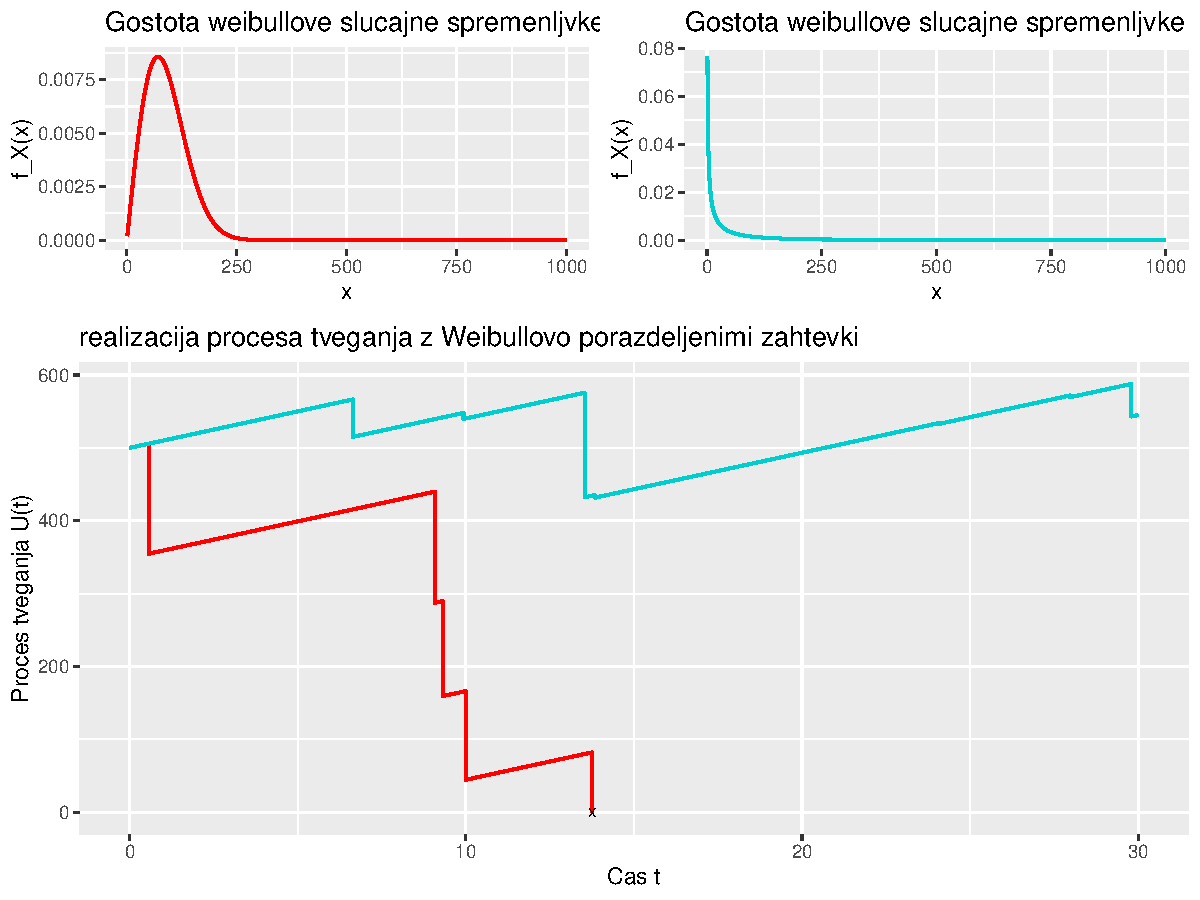
\includegraphics[width=\textwidth]{
                    C:/Users/38651/OneDrive - Univerza v Ljubljani/Desktop/Diploma/Diplomski-seminar/GraphsAndPhotos/slika2.pdf
                    }
                \caption{Realizaciji procesa tveganja}
                \label{fig:slika3}
            \end{figure}

            \noindent
            Pri obeh realizacijah vidimo, da proces tveganja v nekem trenutku pade pod $0$ (tam ga 
            tudi ustavimo). "Ceprav je pri"cakova vrednost 
            $\E\left[Y_i\right] = 384 \approx \E\left[X_i\right] = 217\sqrt{\pi} \approx 384,62$ 
            opazimo bistveno razliko med realizacijama. V rde"cem primeru proces pade pod
            $0$ po ve"c zaporednih manj"sih izgubah, v modrem primeru pa po eni zelo veliki izgubi. 
            V nadaljevanju bomo primera lo"cili, ampak pred tem 
            definirajmo osnovne pojme, ki jih bomo obravnavali v razdelku.

            \label{zgd:weibullProcesTveganja}
        \end{zgled}

        \begin{definicija}
            \textit{Propad} definiramo kot dogodek, da proces tveganja $(U_t)_{t\geq0}$ kadarkoli pade pod $0$. 
            Torej 
            \begin{align*}
                \bigl\{U_t<0 \ \text{za} \ t\geq 0\bigr\}
            \end{align*}
            in "casu ustavljanja
            \begin{align*}
                T = \inf\{t\geq0 \mid U_t < 0\}, 
            \end{align*}
            pravimo \textit{"cas propada}. Seveda velja enakost med dogodkoma
            \begin{align*}
                \{U_t<0 \ \text{za} \ t\geq0\} = \{T<\infty\}.
            \end{align*}
            \label{def:PropadCasPropada} 
        \end{definicija}

        \begin{definicija}
            \textit{Verjetnost propada} je definirana kot funckija $\psi(u): (0,\infty) \to [0,1]$ 
            podana s predpisom
            \begin{align*}
                \psi(u) = \Prob(T<\infty \mid U_0 = u).
            \end{align*}
            \label{def:VerjetnostPropada}
        \end{definicija}

        \begin{definicija}
            Po konstrukciji procesa tveganja $(U_t)_{t\geq0}$ je verjentost propada mogo"ca le ob 
            prihodih zahtevkov. %, ki sledijo $HPP(\lambda)$
            Z $V_n$ ozna"cimo "cas $n$-tega prihoda in definiramo 
            \textit{ogrodje procesa tveganja} kot $(U_{V_n})_{n\in\N}$.
            \label{def:ogrodjeProcesaTveganja}
        \end{definicija}

        \begin{trditev}
            Naj bo $(U_t)_{t\geq0}$ proces tveganja v Cramér-Lundbergovem modelu in $(U_{V_n})_{n\in\N}$ 
            njegovo ogrodje ter $T_n := V_n - V_{n-1}$ medpirhodni "cas $n$-tega zahtevka 
            $(V_0 = T_0 = 0)$. Potem velja 
            \begin{equation*}
                \psi(u) = \Prob\left(\sup_{n\in\N}Z_n > u\right),
            \end{equation*}
            kjer je $Z_n = \sum_{i=1}^nY_i$  komulativna izguba po $n$ prihodih in $Y_i = X_i - cT_i$
            izguba $i$-tega prihoda.
            \label{trd:verjetnostPropadaZOgrodjem}
        \end{trditev}

        \begin{proof}

            S pomo"cjo ogrodja procesa tveganja lahko dogodek propada zapi"semo kot
            \begin{align*}
                \bigl\{U_t<0 \ \text{za} \ t\geq 0\bigr\} &= 
                                \biggl\{\inf_{t\geq0}U_t<0\biggr\} \\
                              &= \biggl\{\inf_{n\in\N}U_{V_n}<0\biggr\} \\
                              &= \biggl\{\inf_{n\in\N}\bigl\{u + p(V_n) - S_{V_n}\bigr\} < 0\biggr\} \\
                              &= \biggl\{\inf_{n\in\N}\biggl\{u + 
                              \underbrace{cV_n - \sum_{i=1}^nX_i}_{-Z_n}\biggr\} < 0\biggr\} \\
                              &= \biggl\{\inf_{n\in\N}\{-Z_n\} < -u\biggr\} \\
                              &= \biggl\{\sup_{n\in\N}Z_n > u\biggr\},
            \end{align*}
            kar nam da "zeljeno enakost.
        \end{proof}

        Tako verjetnost propada prevedemo na prehodno verjetnost diskretnega slu"cajnega 
        sprehoda $(Z_n)_{n\in\N}$. V nadaljevanju nas bo predvsem zanimalo asimptoti"cno 
        vedenje $\psi(u)$, ko gre $u\rightarrow\infty$. Cilj obravnavanja verjetnosti propada v 
        Cramér-Lundbergovem modelu je, da se izognemo skoraj gotovemu propadu oziroma, da je verjetnost, 
        da komulativna izguba $(Z_n)_{n\in\N}$ prese"ze $u$
        tako majhna, da lahko v praksi dogodek propada izklju"cimo. 

        \begin{trditev}
            Naj bo $(Z_n)_{n\in\N}$ zaporedje slu"cajnih spremenljivk definirano kot 
            $Z_n = \sum_{i=1}^nY_i$ za neodvisne in enako porazdeljene slu"cajne spremenljivke 
            $Y_i$ z $\E\left[Y_i\right] < \infty$. 
            "Ce velja $\E\left[Y_i\right] \geq 0$, potem za vsak $u>0$ velja
            \begin{equation*}
                \Prob\left(\sup_{n\in\N}Z_n > u\right) = 1.
            \end{equation*}
            \label{trd:propadZVerjetnostjo1}
        \end{trditev}

        \begin{proof}
            Zaporedje slu"cajnih spremenljivk $(Y_i)_{i\in\N}$ zado"s"ca predpostavkam krepkega zakona
            velikih "stevil (\ref{izr:KrepkiZakonVelikihStevil}), torej velja
            \begin{equation*}
                \frac{Y_1 + Y_2 + \cdots Y_n}{n} = \frac{Z_n}{n} \xrightarrow[n\to\infty]{s.g.} \E\left[Y_n\right].
            \end{equation*}
            Torej bo $Z_n$ v primeru ko je $\E\left[Y_n\right]>0$
             skoraj gotovo asimptoti"cno linearno nara"scal proti $\infty$ kot $\E\left[Y_n\right] n$ in 
             bo za poljuben $u>0$
            \begin{equation*}
                \Prob\left(\sup_{n\in\N}Z_n > u\right) = 1.
            \end{equation*}
            Dokaz za primer, ko je $\E\left[Y_n\right] = 0$ je precej bolj tehni"cen in ne preve"c informativen, zato 
            ga bomo izpustili. Izka"ze se, da obstajata neki podzaporedji$(n_k)_{k\in\N}$ in $(m_k)_{k\in\N}$, da 
            $Z_{n_k} \xrightarrow[k\to\infty]{s.g.}\infty$ in 
            $Z_{m_k} \xrightarrow[k\to\infty]{s.g.}-\infty$.
            Dokaz lahko najdemo v \cite{6}.
        \end{proof}

        \begin{opomba}
            Iz trditve \ref{trd:propadZVerjetnostjo1} (ob predpostavkah $\E\left[X_i\right] < \infty$
            in $\E\left[T_i\right] < \infty$) sledi, da moramo premijo (in s tem $c$) izbrati tako, da bo 
            $\E\left[Y_i\right] < 0$, saj bo tako $Z_{n} \xrightarrow[n\to\infty]{s.g.}-\infty$
            in je to edini primer, ko lahko upamo, da verjetnost propada ne bo
            enaka 1.
            \label{op:izbiraPremije}
        \end{opomba}
    
        %V nadaljevanju bomo
        %predpostavili, da sta $\E\left[X_n\right]$ in $\E\left[W_n\right]$ kon"cni. To nam 
        %zagotovi, da je $\E\left[Z_n\right] = \sum_{i=1}^n\E\left[X_i\right] - c\E\left[W_i\right]$
        %kon"cna.
%
        %Ker pa velja ena od treh mo"znosti:
        %\begin{align*}
        %    \E\left[Y_n\right] = 
        %    \begin{cases}
        %        > 0, & \text{za} \ c\E\left[W_n\right] > \E\left[X_n\right], \\
        %        = 0, & \text{za} \ c\E\left[W_n\right] = \E\left[X_n\right], \\
        %        < 0, & \text{za} \ c\E\left[W_n\right] < \E\left[X_n\right],
        %    \end{cases}
        %\end{align*}
%
        %\noindent
        %bo verjetnost propada enaka 1, "ce velja $\E\left[Y_n\right] > 0$, saj $(Z_n)_{n\in\N}$ 
        %zado"s"ca predpostavkam krepkega zakona velikih "stevil.
        %\begin{equation*}
        %    \frac{Z_n}{n} \xrightarrow[n\to\infty]{s.g.} \E\left[Y_n\right] > 0.
        %\end{equation*}
        %Vidimo torej, da bo $Z_n$ skoraj gotovo linearno nara"scal proti $\infty$ in bo za poljuben 
        %$u>0$
        %\begin{equation*}
        %    \Prob\left(\sup_{n\in\N}Z_n > u\right) = 1.
        %\end{equation*}
%
        %Izka"ze se da celo v 
        %primeru ko bo $\E\left[Y_n\right] = 0$ bo verjetnost propada enaka 1, ker bosta obstajali 
        %pozdaporedji $(n_k)_{k\in\N}$ in $(m_k)_{k\in\N}$... Spitzer [138] je dokazano.

        \begin{definicija}
            Pravimo, da proces tveganja $(U_t)_{t\geq0}$ v Cramér-Lundbergovem modelu
             zado"s"ca \textit{pogoju neto zaslu"zka} (ang. \textit{net profit condition}), "ce velja 
            \begin{equation*}
                c > \frac{\E\left[X_1\right]}{\E\left[T_1\right]}, \quad \text{oziroma} \quad 
                c = (1 + \rho)\frac{\E\left[X_1\right]}{\E\left[T_1\right]} \quad \text{za $\rho > 0$}.
            \end{equation*}
            Pogoj bomo v nadaljenvanju imenovali NPC.
            \label{def:NPC}
        \end{definicija}

        Zahteva NPC za analizo poslovanja zavarovalnice je kar intuitivna, saj pove, da mora  
        biti v nekem "casovnem intervalu pri"cakovan dohodek iz premij ve"cji od pri"cakovanega izpla"cila zahtevkov.

        \begin{definicija}
            Pravimo, da ima slu"cajna spremenljivka $X$ \textit{lahkorepo porazdelitev}, "ce za 
            nek $\varepsilon > 0$ velja
        \begin{equation*}
            \E\left[e^{uX}\right] = M_X(u) < \infty \quad \text{za} \ u \in (-\varepsilon, \varepsilon).
        \end{equation*}
        Sicer $M_X(u)$ obstaja le za $u\in(-\infty, 0]$ in pravimo, 
        da ima $X$ \textit{te"zkorepo porazdelitev}.
        \label{def:lahkorepnaPorazdelitev}
        \end{definicija}

        \begin{zgled}[Nadaljevnaje zgleda \ref{zgd:weibullProcesTveganja}]
            V zgledu \ref{zgd:weibullProcesTveganja} smo obravnavali proces tveganja v Cramér-Lundbergovem 
            modelu, kjer so zahtevki (rde"ca) $X_i\sim\text{Weibull}(2, 434)$ in (modra) 
            $Y_i\sim\text{Weibull}(\tfrac{1}{4}, 16)$. Opazili smo, da je v prvem primeru propad
            posledica ve"c manj"sih izgub, v drugem pa ene velike izgube. To je zna"cilnost te"zkorepih
            porazdelitev in za Weibullovo porazdelitev velja, da ima za parameter
            $a \geq 1$ lahek, za $a<1$ pa te"zek rep.
            \begin{proof}
                Momentno rodovna funkcija $X\sim\text{Weibull}(a, b)$ je enaka
                \begin{align*}
                    M_X(u) &= \int_{0}^{\infty}e^{ux}\frac{a}{b}\left(\frac{x}{b}\right)^{a-1}e^{-\left(\frac{x}{b}\right)^a}dx \qquad \left(y = \tfrac{x}{b},\ dy = \tfrac{dx}{b}\right) \\
                           &= a\int_{0}^{\infty}e^{uby} y^{a-1}e^{-y^a}dy.
                \end{align*}
                Vidimo, da v $0$ ni te"zav za poljuben $a > 0$, ampak za $a\in(0, 1)$ v neskon"cnosti funkcija 
                divergira, saj se 
                eksponent poenostavi v $y^a(uby^{1 - a} - 1)\xrightarrow{y\to\infty}\infty$ ."Ce v 
                nadaljevanju predpostavimo $a\geq 1$ in uvedemo $z = y^a$ 
                $\bigl(dz = ay^{a-1}dy\bigr)$ pa lahko pridemo do lepe oblike 
                za momentno rodovno funkcijo $X$. \phantom{\qedhere}
                \begin{align*}
                    M_X(u) &= \int_{0}^{\infty}e^{ubz^{\frac{1}{a}}}e^{-z}dz \\
                           &= \int_{0}^{\infty}\sum_{k=0}^{\infty}\frac{(ubz^{\frac{1}{a}})^k}{k!}e^{-z}dz \qquad \qquad \text{Tonelli} \ (\ref{izr:TonellijevIzrek}) \\
                           &= \sum_{k=0}^{\infty}\frac{(ub)^k}{k!}\int_{0}^{\infty}z^{\frac{k}{a}}e^{-z}dz \\
                           &= \sum_{k=0}^{\infty}\frac{(ub)^k}{k!}\Gamma\left(\frac{k}{a} + 1\right).
                \end{align*} 
            \end{proof}
            \label{zgd:weibullLahkorepnaPorazdelitev}
        \end{zgled}
    
    \subsection{Lahkorepe porazdelitve}
        Od sedaj naprej bomo predpostavili, da je $(S_t)_{t\geq0}$ v procesu tveganja $(U_t)_{t\geq0}$ $CPP$.
        Najprej se bomo omejili na primer, ko ima porazdelitev slu"cajnih spremenljivk $X_i$, ki jih 
        se"stevamo v $CPP$ lahek rep, saj je bila osnovna teorija, ki sta jo razvila Cramér in Lundberg,
        izpeljana pod to predpostavko.
        \subsubsection{Lundbergova neenakost}

            \begin{opomba}
                V praksi z lahkorepnimi porazdelitvami modeliramo zahtevke, kjer verjentosti ekstremnih 
                dogodkov (torej zelo velikih zahtevkov) eksponentno pada proti $0$. To neposredno sledi iz 
                definicije \ref{def:lahkorepnaPorazdelitev} in neenakosti Markova (\ref{trd:neenakostMarkova}), 
                saj za vsak 
                $x>0$ in $u\in(-\varepsilon, \varepsilon)$ velja
                \begin{equation*}
                    \Prob\left(X > x\right) = \Prob\left(e^{uX} > e^{ux}\right) \leq \frac{\E\left[e^{uX}\right]}{e^{ux}}.
                \end{equation*}
                \label{op:lahkorepnaPorazdelitev}
            \end{opomba}

            \begin{definicija}
                Naj velja, da ima slu"cajna spremenljivka $Y_1 = X_1 - cT_1$ iz trditve \ref{trd:verjetnostPropadaZOgrodjem} 
                lahek rep. "Ce obstaja enoli"cen $\ell > 0$ za katerega velja
                \begin{equation*}
                    M_{Y_1}(\ell)  = 1,
                \end{equation*}
                potem $\ell$ pravimo \textit{Lundbergov koeficient}.
                \label{def:LundbergovKoeficient}
            \end{definicija}

            \begin{trditev}
                "Ce Lundbergov koeficient $\ell$ (pod predpostvakami definicije \ref{def:LundbergovKoeficient} in 
                pogoja NPC)
                obstaja, potem je enoli"cno dolo"cen.
                \label{trd:enolicnostLundbergovegaKoeficienta}
            \end{trditev}

            \begin{proof}
                Ker ima $Y_1$ lahek rep, obstaja $\varepsilon > 0$, da je $M_{Y_1}(u) < \infty$ za $u\in(-\varepsilon, \varepsilon)$.
                Ker velja $M_{Y_1}(0) = 1$ in $M_{Y_1}'(0) = \E\left[Y_1\right] < 0$ (zaradi pogoja NPC) ter
                $M_{Y_1}''(u) = \E\left[Y_1^2e^{Y_1u}\right] > 0$ $(Y_1 \neq 0 \ \text{skoraj gotovo})$ za 
                $u>0$, je $M_{Y_1}(u)$ zvezna konveksna funkcija na intervalu $(-\varepsilon, \varepsilon)$, kjer 
                v okolici ni"cle pada. Po predpostavki obstaja $\ell > 0$, da je $M_{Y_1}(\ell) = 1$, ki pa
                je zaradi konveksnosti funkcije enoli"cno dolo"cen.
            \end{proof}

            \begin{izrek}(Lundbergova neenakost)
                Naj bo $(U_t)_{t\geq0}$ proces tveganja v Cramér-Lundbergovem modelu, ki zado"sca NPC in 
                naj zanj obstaja Lundebrgov koeficient $\ell$. Potem za vsak $u>0$ velja
                \begin{equation*}
                    \psi(u) \leq e^{-\ell u}.
                \end{equation*}
                \label{izr:LundbergovaNeenakost}
            \end{izrek}

            \begin{proof}
                Neenakost bomo dokazali z indukcijo. Za $u>0$ in $n\in\N$ definiramo
                \begin{equation*}
                    \psi_n(u) = \Prob\left(\max_{1\leq k\leq n}Z_k > u\right)
                \end{equation*}
                in vidimo, da je (po zveznosti $\mathbb{P}$ od spodaj) $\psi(u) = \lim_{n\to\infty}\psi_n(u)$, 
                torej moramo pokazati, da za vsak $n\in\N$ velja $\psi_n(u) \leq e^{-\ell u}$. \\
                (n = 1): Uporabimo neenakost Markova in dobimo
                \begin{equation*}
                    \psi_1(u) = \Prob\left(e^{\ell Z_1} > e^{\ell u}\right) \leq \frac{M_{Z_1}(\ell)}{e^{\ell u}} = e^{-\ell u}.
                \end{equation*}
                (n $\rightarrow$ n+1): 
                S $F_{Y_1}$ ozna"cimo porazdeliltev $Y_1$. Potem velja
                \begin{align*}
                    \psi_{n+1}(u) &= \Prob\left(\max_{1\leq k\leq n+1}Z_k > u\right) \\
                                  &= \underbrace{\Prob\left(Y_1 > u\right)}_{(i)} + 
                                  \underbrace{\Prob\left(\max_{2\leq k\leq n+1}\bigl\{Y_1 + (Z_k - Y_1)\bigr\} > u, Y_1 \leq u\right)}_{(ii)} \\
                \end{align*}
                Najprej se posvetimo $(ii)$. Po indukcijski predpostavki velja 
                \begin{align*}
                    (ii) &= \int_{(-\infty, u]}\Prob\left(\max_{1\leq k\leq n}\bigl\{x + Z_k\bigr\} > u\right)dF_{Y_1}(x) \\
                         &= \int_{(-\infty, u]}\Prob\left(\max_{1\leq k\leq n}Z_k > u - x\right)dF_{Y_1}(x) \\
                         &= \int_{(-\infty, u]}\psi_n(u - x)dF_{Y_1}(x) \\
                         &\stackrel{\text{\scalebox{0.8}{I.P.}}}{\leq} \int_{(-\infty, u]}e^{-\ell(u - x)}dF_{Y_1}(x). \\
                \end{align*}
                Za oceno $(i)$ kot v primeru $n=1$ uporabimo neenakost Markova in dobimo

                \begin{equation*}
                    (i) = \psi_1(u) \leq \frac{M_{Z_1}(\ell)}{e^{\ell u}} = \int_{(u, \infty)}e^{-\ell (u-x)}dF_{Y_1}(x).
                \end{equation*}
                "Ce torej se"stejemo $(i)$ in $(ii)$ dobimo "zeljeno oceno

                \begin{align*}
                    \psi_{n+1}(u) &\leq \int_{\R}e^{-\ell (u - x)}dF_{Y_1}(x) \\
                                  &= e^{-\ell u}M_{Y_1}(\ell) \\
                                  &= e^{-\ell u}.
                \end{align*}

            \end{proof}

            \begin{opomba}
                Iz izreka \ref{izr:LundbergovaNeenakost} je razvidno, da z dovolj visokim za"cetnim kapitalom
                $u$ verjetnost propada lahko v praksi zadovoljivo omejimo blizu $0$. Seveda je meja 
                odvisna tudi od Lundbergovega koeficienta $\ell$ in krepko temelji na predpostavki 
                lahkorepnih porazdelitev, ki pa v praksi pogosto niso izpolnjene.
                \label{op:LundbergovaNeenakost}
            \end{opomba}

            \begin{zgled}
                Naj bo $(U_t)_{t\geq0}$ proces tveganja v Cramér-Lundbergovem modelu, ki zado"s"ca NPC.\ Naj 
                nadalje velja da so zahtevki neodvisno eksponentno porazdeljeni s parametrom $\mu > 0$, torej 
                $X_i \stackrel{\text{\scalebox{0.8}{n.e.p.}}}{\sim} \text{Exp}(\mu) \ \text{za vsak} \ i$. Vemo, da ima momentno rodovna funkcija 
                $X_i$ obliko 

                \begin{equation*}
                    M_{X_i}(u) = \frac{\mu}{\mu - u} \ \text{za} \ u<\mu.
                \end{equation*}
                Tako dobimo, da ima momentno rodovna funkcija $Y_1 = X_1 - cT_1$ obliko 

                \begin{equation*}
                    M_{Y_1}(u) = M_{X_1}(u)M_{T_1}(-cu) = 
                    \frac{\mu}{\mu - u}\frac{\lambda}{\lambda + cu} \ \text{za} \ u\in (-\tfrac{\lambda}{c}, \mu).
                \end{equation*}
                Sedaj lahko izra"cunamo Lundbergov koeficient $\ell$

                \begin{align*}
                    M_{Y_1}(\ell) &= 1, \\
                    \frac{\mu}{\mu - \ell}\frac{\lambda}{\lambda + c\ell} &= 1, \\
                    \mu\lambda &= (\mu - \ell)(\lambda + c\ell), \\
                    \mu\lambda &= \mu\lambda - \ell\lambda + \mu c - c\ell^2, \\
                    0 &= \mu c - c\ell - \lambda.
                \end{align*}
                Dobimo 
                \begin{equation}
                    \ell = \mu - \frac{\lambda}{c}.
                    \label{eq:LundbergovKoeficientExpPrva}
                \end{equation}
                Velja $\ell \in (0, \mu)$, saj v na"sem modelu velja pogoj NPC,
                \begin{equation*}
                    \frac{\E\left[X_1\right]}{\E\left[T_1\right]} = \frac{\lambda}{\mu} < c \iff \mu > \frac{\lambda}{c}.
                \end{equation*}
                "Ce uporabimo alternativno formulacijo NPC pogoja, dobimo
                \begin{equation}
                    c = (1 + \rho)\frac{\lambda}{\mu} \quad \Rightarrow \quad
                    \ell = \mu - \frac{\lambda}{(1 + \rho)\frac{\lambda}{\mu}} = \mu\left(\frac{\rho}{1 + \rho}\right).
                    \label{eq:LundbergovKoeficientExp}
                \end{equation}
                Tako dobimo zgornjo mejo za verjetnost propada
                \begin{equation*}
                    \psi(u) \leq e^{-\ell u} = e^{-\mu u\left(\frac{\rho}{1 + \rho}\right)}
                \end{equation*}
                in vidimo, da pove"canje stopnje prihodkov premij "cez neko mejo ne bistveno 
                vpliva na oceno, saj 
                \begin{equation*}
                    \lim_{\rho\to\infty}e^{-\mu u\left(\frac{\rho}{1 + \rho}\right)} = e^{-\mu u}.
                \end{equation*}
                V nadaljevanju bomo videli, da je Lundbergova neenakost v primeru eksponentno 
                porazdeljenih zahtevkov skoraj to"cna vrednost verjetnosti propada, zgre"sena le za konstanto.
                V splo"snem pa je zelo te"zko dolo"citi Lunbergov koeficient kot funkcijo parametrov
                porazdelitev $X_1$ in $T_1$ in zato uporabljamo numeri"cne metode za njegovo aproksimacijo 
                kot na primer Monte Carlo simulacije. 
                \label{zgd:LundebrgovaNeenakostEksponentno}
            \end{zgled}

        \subsubsection{Asimptotika verjetnosti propada}
            Sedaj se posvetimo vpra"sanju, kako se obna"sa verjetnost propada v Cramér-Lundbergovem modelu,
            ko gre $u\rightarrow\infty$ in izpeljemo enega temeljnih rezultatov v teoriji tveganja.

            \begin{definicija}
                Za la"zjo notacijo v nadaljevanju definiramo funkcijo \textit{verjentosti pre"zivetja} kot
                $\theta(u):(0, \infty) \to [0, 1]$ s predpisom
                \begin{equation*}
                    \theta(u) = \Prob\left(T=\infty\mid U_0=u\right) = 1 - \psi(u).
                \end{equation*}
                \label{def:verjetnostPrezivetja}
            \end{definicija}

            \begin{lema}(Integralska ena"cba za verjetnost pre"zivetja)
                Naj bo $(U_t)_{t\geq0}$ proces tveganja v Cramér-Lundbergovem modelu, ki zado"s"ca NPC in naj 
                velja $\E\left[X_1\right]<\infty$ ter, da imajo slu"cajne spremenljivke $(X_i)_{i\in\N}$ 
                gostoto. Potem $\theta(u)$ zado"sca naslednji enakosti
                \begin{equation}
                    \theta(u) = \theta(0) + \frac{1}{(1+\rho)\E\left[X_1\right]} \int_{(0, u]}\bigl(1 - F_{X_1}(x)\bigr)\theta(u - x)dx.
                    \label{eq:verjetnostPrezivetja}
                \end{equation}
                \label{lema:verjetnostPrezivetja}
            \end{lema}

            \begin{proof}
                Po trditvi \ref{trd:verjetnostPropadaZOgrodjem} velja
                \begin{equation*}
                    \psi(u) = \Prob\left(\sup_{n\in\N}Z_n > u\right),
                \end{equation*}
                kjer je $Z_n = \sum_{i=1}^nY_i$ in $Y_i = X_i - cT_i$. Torej je
                \begin{align*}
                    \theta(u) &= \Prob\left(\sup_{n\in\N}Z_n \leq u\right) \\
                              &= \Prob\biggl(\bigl\{Z_n \leq u\mid n\in\N\bigr\}\biggr) \\
                              &= \Prob\biggl(\bigl\{Y_1 \leq u\bigr\}\cap \bigl\{Z_n - Y_1 \leq u - Y_1\mid n\geq2\bigr\}\biggr) \\
                              &= \E\biggl[\mathbbm{1}_{\{Y_1\leq u\}}\Prob\biggl(\bigl\{Z_n - Y_1 \leq u - Y_1\mid n\geq2\bigr\} \ \Big| \ Y_1\biggr)\biggr].
                \end{align*}
                Sedaj upo"stevamo, da je $Y_1 = X_1 - cT_1$ in je torej dogodek $\{Y_1 \leq u\}$ 
                enak dogodku $\{X_1 \leq u + cT_1\}$. Poleg tega velja, da je 
                $(Z_n - Y_1)_{n\geq2} \sim (Z_n)_{n\in\N}$, saj so $Y_i$ neodvisne in enako porazdeljene
                slu"cajne spremenljivke.
                Upo"stevamo "se, da je  $T_1$ medprihodni "cas v $HPP(\lambda)$ da dobimo

                \begin{align*}
                        \theta(u)   &= \int_{(0, \infty)}\int_{(0, u + ct]}\Prob\biggl(\bigl\{Z_n \leq u - (x - ct)\mid n\in\N\bigr\}\biggr)dF_{X_1}(x)dF_{T_1}(t) \\
                                    &= \int_{(0, \infty)}\int_{(0, u + ct]}\theta(u - x + ct)dF_{X_1}(x)\lambda e^{-\lambda t}dt.
                \end{align*}
                Uvedemo novo spremenljivko $z = u + ct$ $\bigl( \text{torej} \ t = \tfrac{z - u}{c}$ in $dt = \tfrac{dz}{c} \bigr)$ 
                in dobimo

                \begin{align*}
                            \theta(u) = \frac{\lambda}{c}e^{\frac{\lambda u}{c}}\int_{(u, \infty)}e^{-\frac{\lambda z}{c}}\underbrace{\int_{(0, z)}\theta(z - x)dF_{X_1}(x)}_{g(z)}dz.
                \end{align*}
                Ker ima porazdelitev $F_{X_1}$ gostoto in je $\theta$ zvezna omejena funkcija,
                je funkcija $g(z)$ zvezna in jo lahko (po osnovnem izreku analize)
                odvajamo da dobimo

                \begin{equation*}
                    \theta'(u) = \frac{\lambda}{c}\theta(u) - \frac{\lambda}{c}\int_{(0, u)}\theta(u - x)dF_{X_1}(x).
                \end{equation*}
                "Ce sedaj obe strani integriramo po $u$ dobimo
                
                \begin{equation}
                    \int_{(0, t]}\theta'(u)du = \frac{\lambda}{c}\int_{(0, t]}\theta(u)du - \overbrace{\frac{\lambda}{c}\int_{(0, t]}\underbrace{\int_{(0, u]}\theta(u - x)dF_{X_1}(x)}_{(i)}du.}^{(ii)} 
                    \label{eq:verjetnostPrezivetjaIntegral}
                \end{equation}
                Na integralu $(i)$ uporabimo per partes $\bigl(\alpha = \theta(u-x)$ in $d\beta = dF_{X_1}(x)\bigr)$ 
                ter upo"stevamo, da ima $F_{X_1}$ gostoto.

                \begin{align*}
                    (i)     &= \bigl(\theta(u - x)F_{X_1}(x)\bigr)\Big|_{0}^{u} + \int_{(0, u)}\theta'(u - x)F_{X_1}(x)dx \\
                            &= \theta(0)F_{X_1}(u) - \int_{(0, u)}\theta'(u - x)F_{X_1}(x)dx.
                \end{align*}
                Upo"stevamo, da je $F_{X_1}(0) = 0$, saj je $X_1 > 0$ skoraj gotovo. Vstavimo $(i)$ 
                v $(ii)$ in dobimo

                \begin{equation*}
                    (ii) =  - \frac{\lambda}{c}\int_{(0, t]}\theta(0)F_{X_1}(u)du - \frac{\lambda}{c}\int_{(0, t]}\int_{(0, u]}\theta'(u - x)F_{X_1}(x)dxdu. 
                \end{equation*}
                Po Tonellijevem izreku (\ref{izr:TonellijevIzrek}) lahko zamenjamo vrstni red integracije.

                \begin{align*}
                    (ii)    &=  - \frac{\lambda}{c}\int_{(0, t]}\theta(0)F_{X_1}(u)du - \frac{\lambda}{c}\int_{(0, t]}F_{X_1}(x)\int_{[x, t]}\theta'(u - x)dudx \\
                            &= - \frac{\lambda}{c}\int_{(0, t]}\theta(0)F_{X_1}(u)du - \frac{\lambda}{c}\int_{(0, t]}F_{X_1}(x)\bigl(\theta(t-x) - \theta(0)\bigr)dx.\\
                            &= - \frac{\lambda}{c}\int_{(0, t]}F_{X_1}(x)\theta(t - x)dx.
                \end{align*}
                Vstavimo $(ii)$ v ena"cbo (\ref{eq:verjetnostPrezivetjaIntegral}) in dobimo
                \begin{align*}
                    \theta(t) - \theta(0) &= \frac{\lambda}{c}\int_{(0, t]}\theta(u)du - \frac{\lambda}{c}\int_{(0, t]}F_{X_1}(x)\theta(t - x)dx,\\
                    \theta(t) &= \theta(0) + \frac{\lambda}{c}\int_{(0, t]}\bigl(1 - F_{X_1}(x)\bigr)\theta(t - x)dx.
                \end{align*}
                "Ce sedaj upo"stevamo enakost 
                \begin{equation*}
                    \frac{\lambda}{c} = \frac{1}{1 + \rho}\frac{1}{\E\left[X_1\right]}
                \end{equation*}
                in zamenjamo oznako spremenljivke $t\mapsto u$, dobimo "zeljeno enakost (\ref{eq:verjetnostPrezivetja}).

            \end{proof}

            \begin{opomba}
                    Ena"cbo (\ref{eq:verjetnostPrezivetja}) lahko zapi"semo tudi v obliki 
                    \begin{equation}
                        \theta(u) = \theta(0) + \frac{1}{1+\rho}\int_{(0, u]}\theta(u - x)d\overline{F}_{X_1}(x),
                        \label{eq:verjetnostPrezivetja2}
                    \end{equation}
                    kjer je $\overline{F}_{X_1}$ porazdelitev integriranega repa (\ref{def:porazdelitevintegriranegaRepa}) 
                    slu"cajne spremenljivke $X_1$.
                    %Hitro lahko preverimo, da je $F_X^I(x)$ porazdelitvena funkcija, saj je $F_X^I(0) = 0$, 
                    %$F_X^I(x)$ je nara"s"cajo"ca in $F_X^I(x) \uparrow 1$ za $x\to\infty$, ker velja 
                    %$\E\left[X\right] = \int_{(0, \infty)}(1 - F_X(x))dx.$ Po osnovnem izreku analize 
                    %(oz. ker ima $F_X^I(x)$ gostoto) pa 
                    %neposredno sledi enakost med (\ref{eq:verjetnostPrezivetja})
                    %in (\ref{eq:verjetnostPrezivetja2}).
                \label{op:verjetnostPrezivetja1}
            \end{opomba}

            \begin{opomba}
                Konstanto $\theta(0)$, ki se pojavi v (\ref{eq:verjetnostPrezivetja}) in      
                (\ref{eq:verjetnostPrezivetja2}) lahko izra"cunamo. Ker $c$ zado"sca NPC, po argumentu v dokazu trditve
                \ref{trd:propadZVerjetnostjo1} velja 
                \begin{equation*}
                    Z_n \xrightarrow[n\to\infty]{s.g.} -\infty.
                \end{equation*}
                Po zveznosti $\Prob$ od spodaj sledi

                \begin{equation*}
                    \lim_{u\to\infty}\Prob\left(\sup_{n\in\N}Z_n \leq u\right) = \Prob\left(\sup_{n\in\N}Z_n \leq \infty\right) = 1.
                \end{equation*}
                "Ce torej v ena"cbi (\ref{eq:verjetnostPrezivetja2}) po"sljemo $u\to\infty$, dobimo

                \begin{equation*}
                    \lim_{u\to\infty}\theta(u) = 1 = \theta(0) + \frac{1}{1 + \rho}\lim_{u\to\infty}\int_{(0, \infty)}\mathbbm{1}_{(0, u]}(x)\theta(u - x)d\overline{F}_{X_1}(x). \\
                \end{equation*}
                Po izreku o monotoni konvergenci (\ref{izr:monotonaKonvergenca}) sledi

                \begin{align*}
                    1 &= \theta(0) + \frac{1}{1 + \rho}\int_{(0, \infty)}1d\overline{F}_{X_1}(x) \\
                     &= \theta(0) + \frac{1}{1 + \rho}.
                \end{align*}
                Torej je $\theta(0) = \frac{\rho}{1 + \rho}$.
                Enakost upo"stevamo v ena"cbi (\ref{eq:verjetnostPrezivetja2}) in dobimo

                \begin{equation}
                    \theta(u) = \frac{\rho}{1 + \rho} + \frac{1}{1 + \rho}\int_{(0, u]}\theta(u - x)d\overline{F}_{X_1}(x).
                    \label{eq:verjetnostPrezivetja3}
                \end{equation}
                %in pomembneje
                %\begin{equation}
                %    \psi(u) = \frac{\rho}{1 + \rho} - \frac{1}{(1 + \rho)\E\left[X\right]}\int_{(0, u]}\bigl(1 - F_X(x)\bigr)\theta(u - x)dx.
                %\end{equation}

                \label{op:verjetnostPrezivetja2}
            \end{opomba}

            \begin{izrek}(Asimptotika verjetnosti propada, lahkorepe porazdelitve)
                Naj bo $(U_t)_{t\geq0}$ proces tveganja v Cramér-Lundbergovem modelu, ki zado"s"ca NPC in 
                naj zanj obstaja Lundbergov koeficient $\ell$. Naj imajo slu"cajne spremenljivke 
                $(X_i)_{i\in\N}$ gostoto.\ Potem obstaja konstanta $C>0$ da
                velja 
                \begin{equation*}
                    \lim_{u\to\infty}e^{\ell u}\psi(u) = C.
                \end{equation*}
                \label{izr:CramerjevaMeja}
            \end{izrek}

            \begin{proof} 
                Najprej preoblikujemo ena"cbo (\ref{eq:verjetnostPrezivetja3}), tako da 
                upo"stevamo $\theta = 1 - \psi$

                \begin{align*}
                    1 - \psi(u) &= \frac{\rho}{1 + \rho} + \frac{1}{1 + \rho}\int_{(0, u]}\bigl(1 - \psi(u - x)\bigr)d\overline{F}_{X_1}(x), \\
                    \psi(u) &= \frac{1}{1 + \rho}\bigl(1 - \overline{F}_{X_1}(u)\bigr) + \frac{1}{1 + \rho}\int_{(0, u]}\psi(u - x)d\overline{F}_{X_1}(x).
                \end{align*}
                Za la"zjo notacijo uvedemo oznako $q = \frac{1}{1 + \rho}$ in dobimo

                \begin{equation}
                    \psi(u) = q\bigl(1 - \overline{F}_{X_1}(u)\bigr) + \int_{(0, u]}\psi(u - x)d\bigl(q\overline{F}_{X_1}(x)\bigr).
                    \label{eq:verjetnostPropadaQ}
                \end{equation}
                Vidimo, da ima ena"cba (\ref{eq:verjetnostPropadaQ}) obliko prenovitvene 
                ena"cbe (\ref{def:prenovitvenaEnacba}) z bistveno razliko, da $q\overline{F}_{X_1}$ ni
                verjetnostna mera, saj velja $\lim_{x\to\infty}q\overline{F}_{X_1}(x) = q < 1$. Ena"cbi 
                (\ref{eq:verjetnostPropadaQ}) pravimo defektna prenovitvena ena"cba. Za $x > 0$ 
                definiramo funkcijo $F_\ell$ kot Esscherjevo transformacijo funkcije $q\overline{F}_{X_1}$.
                \begin{equation*}
                    F_\ell(x) = \int_{(0, x]}e^{\ell y}d\bigl(q\overline{F}_{X_1}(y)\bigr) = \frac{q}{\E\left[X_1\right]}\int_{(0, x]}e^{\ell y}\bigl(1 - F_{X_1}(y)\bigr)dy, 
                \end{equation*}
                Poka"zimo, da je $F_\ell$ porazdelitvena funkcija. O"citno je nara"s"cajo"ca in velja

                \begin{align*}
                    \lim_{x\to\infty}F_\ell(x) &= \frac{q}{\E\left[X_1\right]}\int_{(0, \infty)}e^{\ell y} \bigl(1 - F_{X_1}(y)\bigr)dy \qquad \bigl(\alpha = 1 - F_{X_1}(y), \ d\beta = e^{\ell y}dy\bigr)\\
                                               &= \frac{q}{\E\left[X_1\right]}\biggl(\biggl(\frac{\bigl(1 - F_{X_1}(y)\bigr)e^{\ell y}}{\ell}\biggr)\Big|_{0}^{\infty} + \frac{1}{\ell}\int_{(0, \infty)}e^{\ell y}f_{X_1}(y)dy\biggr) \\
                                               &= \frac{q}{\E\left[X_1\right]}\frac{1}{\ell}\biggl(\E\left[e^{\ell X_1}\right] - 1\biggr).
                \end{align*}
                Sedaj upo"stevamo, da je $q = \frac{1}{1 + \rho} = \frac{\E\left[X_1\right]}{c\E\left[T_1\right]}$ in 
                definicijo Lundbergovega koeficienta ter dejstvo, da je $T_1\sim\text{Exp}(\lambda)$ medprihodni "cas v $\text{HPP}(\lambda)$, da dobimo

                \begin{align*}
                    \lim_{x\to\infty}F_\ell(x)  &= \frac{\E\left[e^{\ell X_1}\right] - 1}{c\ell\ \E\left[T_1\right]}\\
                                                &= \frac{\frac{\lambda + c\ell}{\lambda} - 1}{c\ell \frac{1}{\lambda}} = 1.
                \end{align*}
                "Ce torej ena"cbo (\ref{eq:verjetnostPropadaQ}) pomno"zimo z $e^{\ell u}$, dobimo
                \begin{align}
                    e^{\ell u}\psi(u)   &= qe^{\ell u}\bigl(1 - \overline{F}_{X_1}(u)\bigr) + \int_{(0, u]}e^{\ell (u - x)}\psi(u - x)e^{\ell x}d\bigl(q\overline{F}_{X_1}(x)\bigr) \nonumber \\
                                        &= qe^{\ell u}\bigl(1 - \overline{F}_{X_1}(u)\bigr) + \int_{(0, u]}e^{\ell (u - x)}\psi(u - x)dF_\ell(x). \label{eq:CramérjevaPrenovitvenaEnacba}
                \end{align}
                Vidimo, da sedaj ena"cba (\ref{eq:CramérjevaPrenovitvenaEnacba}) ustreza obliki $\left(qe^{\ell u}\bigl(1 - \overline{F}_{X_1}(u)\bigr), F_\ell\right)$
                prenovitvene ena"cbe in ker je funkcija $qe^{\ell u}\bigl(1 - \overline{F}_{X_1}(u)\bigr)$ omejena na kon"cnih 
                intervalih in $F_\ell$ nearitmeti"cna, lahko uporabimo Smithov klju"cni prenovitveni izrek (\ref{izr:Smith}), da dobimo
                re"sitev
                
                \begin{equation}
                    e^{\ell u}\psi(u) =qe^{\ell u}\bigl(1 - \overline{F}_{X_1}(u)\bigr) +  q\int_{(0, u]}e^{\ell(u - x)}\bigl(1 - \overline{F}_{X_1}(u - x)\bigr)dM^{\ell}(x),
                    \label{eq:resitevCramerjevePrenovitveneEnacbe}
                \end{equation}
                kjer je $M^{\ell}$ prenovitvena mera prenovitvenega procesa z medprihodnimi "casi, 
                ki imajo porazdelitveno funkcijo $F_\ell$. V splo"snem te"zko dolo"cimo $M^{\ell}$, 
                ampak, "ce je $qe^{\ell u}(1 - \overline{F}_X(u))$ direktno Riemannovo integrabilna, nam 
                Smithov izrek da asimptoti"cno vedenje re"sitve (\ref{eq:resitevCramerjevePrenovitveneEnacbe}),
                ko gre $u\to\infty$.
                Direktno Riemannovo integrabilnost preverimo tako, da zapi"semo 
                \begin{align*}
                    qe^{\ell u}(1 - \overline{F}_{X_1}(u)) &= \int_{()}
                \end{align*}
                Tako vidimo, da je $qe^{\ell u}(1 - \overline{F}_{X_1}(u))$ razlika dveh nenara"scajocih
                Riemannovo integrabilnih funkcij in je zato po kriteriju (\ref{trd:kriterijZaDirektnoRiemannovoIntegrabilnost}) 
                direktno Riemannovo integrabilna. Dobimo 
                \begin{equation}
                    C = \lim_{u\to\infty}e^{\ell u}\psi(u) =  \frac{q}{\alpha} \int_{(0, \infty)}e^{\ell x}(1 - \overline{F}_{X_1}(x))dx,
                    \label{eq:CramerBoundConstant}
                \end{equation}
                kjer je $\alpha = \int_{(0, \infty)}x dF_\ell(x)$. S tem je izrek dokazan.
            \end{proof}

            \begin{opomba}
                Izrek \ref{izr:CramerjevaMeja} nam pove, da v primeru zahtevkov z lahkorepimi porazdelitvami verjentost
                propada asimptoti"cno to"cno ekspoenento pada proti $0$ s tem ko za"cetni kapital $u$ raste 
                "cez vse meje.
                
                \label{op:pomenCramerevegaIzreka}
            \end{opomba}

            \begin{zgled}(Nadaljevnaje zgleda \ref{zgd:LundebrgovaNeenakostEksponentno})
                Vemo, da re"sitve prenovitvene ena"cbe (\ref{eq:resitevCramerjevePrenovitveneEnacbe}) 
                iz izreka \ref{izr:CramerjevaMeja} v splo"snem ne moremo izra"cuanti.
                V zgledu \ref{zgd:LundebrgovaNeenakostEksponentno} smo pa privzeli, da zahtevke modeliramo 
                z eksponentno porazdelitvijo, torej $X_i\sim\text{Exp}(\mu)$. 
                V tem primeru se izka"ze, da lahko eksplicitno izra"cunamo verjentost propada.
                "Ce si pogledamo ena"cbo (\ref{eq:resitevCramerjevePrenovitveneEnacbe}), vidimo, da moramo 
                izra"cunati le porazdelitev integriranega repa $\overline{F}_{X_1}(u)$ in 
                prenovitveno mero Esscherjeve transformacije $F_\ell$. Za eksponentno porazdelitev
                velja
                \begin{align*}
                    \overline{F}_{X_1}(u)   &= \frac{1}{\E\left[X_1\right]}\int_{(0, u)}\bigl(1 - F_{X_1}(t)\bigr)dt \\
                                            &= \mu\int_{(0, u)}e^{-\mu t}dt \\
                                            &= F_{X_1}(u),
                \end{align*}
                saj je pozabljiva. Prenovitveno mero Esscherjeve transformacije pa dobimo tako, 
                da prvo izra"cunamo porazdelitveno funckijo $F_\ell$ podano v ena"cbi (\ref{eq:verjetnostPrezivetja2}). 

                \begin{align*}
                    F_\ell(u)  &= \frac{q}{\E\left[X_1\right]}\int_{(0, u]}e^{\ell x}\bigl(1 - F_{X_1}(x)\bigr)dx \\
                            &= \frac{\mu}{1 + \rho}\int_{(0, u]}e^{-x(\mu - \ell)}dx. \\
                \end{align*}
                Upo"stevamo rezultat (\ref{eq:LundbergovKoeficientExp}), torej 
                $\ell = \mu\left(\tfrac{\rho}{1 - \rho}\right)$ in vidimo, da je $F_\ell$ porazdelitvena 
                funkcija eksponentne slu"cajne spremenljvike s paramterom $\frac{\mu}{1 + \rho}$ oziroma 
                $\mu q$. Torej je prenovitvena mera $M^\ell(t)$ preprosto pri"cakovano "stevilo prihodov do 
                "casa $t$ v $\text{HPP}(\mu q)$, torej $M^\ell(t) = \mu qt$.
                "Ce vstavimo rezultata v ena"cbo (\ref{eq:resitevCramerjevePrenovitveneEnacbe}) dobimo
                \begin{align*}
                    e^{\ell u}\psi(u)   &= qe^{\ell u}e^{-\mu u} + q\int_{(0, u]}e^{\ell(u - x)}e^{-\mu(u - x)}dM^\ell(x)\\
                                        &= qe^{-u(\mu - \ell)} + \mu q^2\int_{(0, u]}e^{-(\mu - \ell)(u - x)}dx \\
                                        &= qe^{-u(\mu - \ell)} + \mu q^2 \frac{1}{\mu - \ell}\biggl(1 - e^{-u(\mu - \ell)}\biggr)\\
                                        &= qe^{-u(\mu - \ell)} + \frac{\mu}{(1 + \rho)^2}\frac{1 + \rho}{\mu}\biggl(1 - e^{-u(\mu - \ell)}\biggr) \\
                                        &= qe^{-u(\mu - \ell)} + q\biggl(1 - e^{-u(\mu - \ell)}\biggr) \\
                                        &= q = \frac{1}{1 + \rho}.
                \end{align*}
                Kon"cno dobimo, da je verjetnost propada enaka
                \begin{equation}
                    \psi(u) =  \tfrac{1}{1+\rho}e^{-\ell u}.
                \label{eq:eksplicitnaVerjetnostPropadaExp}
                \end{equation}
            \end{zgled}

                Vidimo, da se $\psi(u)$ z oceno, ki jo dobimo z Lundbergovo neenakostjo v zgledu \ref{zgd:LundebrgovaNeenakostEksponentno} 
                res razlikuje le za konstanto $\tfrac{1}{1 + \rho}$.
                To je seveda zelo poseben primer, ko lahko vse koli"cine izra"cunamo eksplicitno.
                Poka"zimo kako bi do približkov funkcije $\psi(u)$ v praksi lahko pri"sli z Monte 
                Carlo simulacijami.
            
            \begin{zgled}
                Kot v zgledu \ref{zgd:LundebrgovaNeenakostEksponentno} predpostavimo, da so 
                zahtevki porazdeljeni eksponentno, torej $X_i\sim\text{Exp}(\mu)$. Recimo, da je intenzivnost 
                prihodov zahtevkov $\lambda = 1$, stopnja prihodkov premij $c = 1500$ in 
                pri"cakovana vrednost zahtevkov $1000$ \euro, torej 
                $\mu = \tfrac{1}{1000}$. Potem lahko verjetnost propada eksplicitno izra"cunamo po 
                formuli (\ref{eq:eksplicitnaVerjetnostPropadaExp}). Prvo izra"cuamo $\rho$ po formuli
                (\ref{eq:LundbergovKoeficientExp}), in $\ell$ po (\ref{eq:LundbergovKoeficientExpPrva}), torej
                \begin{align*}
                    \rho &= \frac{c\mu}{\lambda} - 1\\
                         &= \frac{1500\cdot\tfrac{1}{1000}}{1} - 1 = \frac{1}{2},
                \end{align*}
                \begin{align*}
                    \ell &= \mu - \frac{\lambda}{c} \\
                         &= \frac{1}{1000} - \frac{1}{1500} = \frac{1}{3000}.
                \end{align*}
                Vsatvimo vrednosti v (\ref{eq:eksplicitnaVerjetnostPropadaExp}) in dobimo
                \begin{equation*}
                    \psi(u) = \tfrac{2}{3}e^{-\frac{u}{3000}}.
                \end{equation*}
                Sedaj definiramo zaporedje $(u_n)_{n = 1}^{50}$ s predpisom $u_n = 500n$ in za vsak $n$
                simuliramo $10, 50$ in $100$ realizacij procesa tveganja, bodisi do "casa $T = 1000$ bodisi dokler
                ne propade in za vsak $n$ izra"cunamo pribli"zek za verjetnost propada kot dele"z propadlih 
                realizacij z vsemi. Aproksimacijo $\psi(u)$ prika"zemo na sliki \ref{fig:slika4}.

                \begin{figure}[H]
                    \centering
                    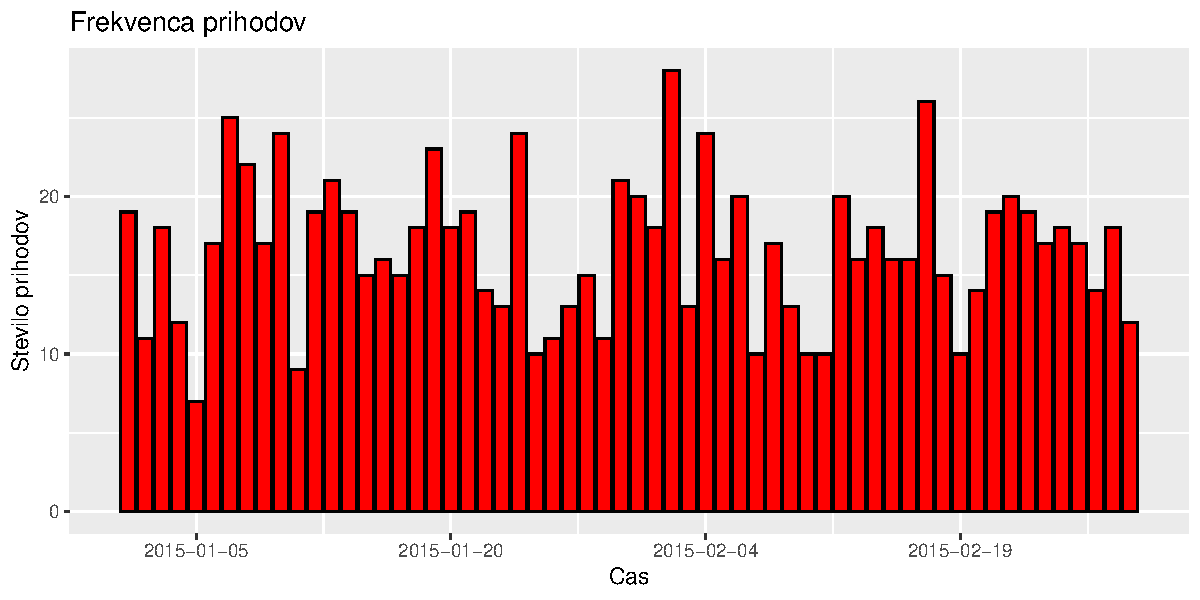
\includegraphics[width=\textwidth]{
                        C:/Users/38651/OneDrive - Univerza v Ljubljani/Desktop/Diploma/Diplomski-seminar/GraphsAndPhotos/slika3.pdf
                        }
                    \caption{Aproksimacija verjetnosti propada $\psi(u)$ z Monte Carlo simulacijami.}
                    \label{fig:slika4}
                \end{figure}

                \noindent
                Kot vidimo, se pribli"zki z nara"s"cajocim "stevilom simulacij prili"zujejo funckciji $\psi(u)$, ampak, za 
                res dobro aproksimacijo, bi morali to "stevilo krepko pove"cati, saj na primer
                za vrednost $u = 16000$ je $\psi(16000) \approx 0.0032186334$, kar je pribli"zno
                $0.3\%$ in v praksi ni zanemarljivo, ampak v na"si simulaciji nobena realizacija procesa 
                tveganja ni padla pod 0.


                %Definiramo "se zaporedje $(\hat{u}_n)_{n = 1}^{25}$ s predpisom $\hat{u}_n = 5000n$ in za vsak $n$
                %izra"cunamo produkt $\psi(\hat{u}_n)e^{\ell \hat{u}_n}$, kjer do ocene za $\psi(\hat{u}_n)$
                %pridemo na enak na"cin kot zgoraj le, da tokrat za posamezno oceno $\psi(\hat{u}_n)$ izvedemo 
                %1000 simulacij, saj je verjetnost propada zelo nizka. Po formuli 
                %(\ref{eq:CramerBoundConstant}) dobimo, da mora $\psi(\hat{u}_n)e^{\ell \hat{u}_n}$ 
                %konvergirati proti
 %
                %\begin{align*}
                %    C       &= \frac{1}{\mu} \int_{(0, \infty)}e^{\ell x}(1 - \overline{F}_{X_1}(x))dx \\
                %            &= 1000 \int_{(0, \infty)}e^{\frac{x}{3000}}\left(1 - (1  - e^{\frac{x}{1000}})\right)dx \\
                %            &= \frac{4}{9000}  \int_{(0, \infty)}e^{-\frac{2x}{3000}}dx \\
                %            &= \frac{2}{3},
                %\end{align*}
                %kar je razvidno, "ze "ce pogledamo (\ref{eq:eksplicitnaVerjetnostPropadaExp}).
                %Rezultate prika"zemo na sliki \ref{fig:slika5}.
%
                %\begin{figure}[H]
                %    \centering
                %    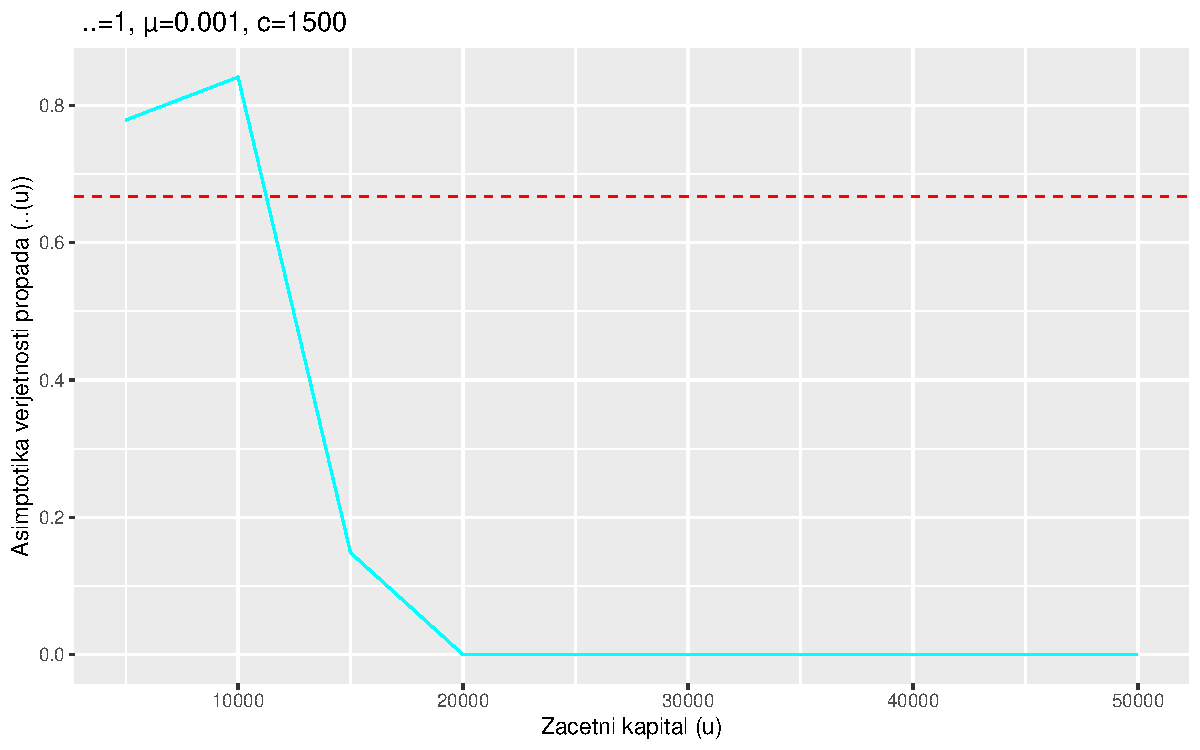
\includegraphics[width=\textwidth]{
                %        C:/Users/38651/OneDrive - Univerza v Ljubljani/Desktop/Diploma/Diplomski-seminar/GraphsAndPhotos/slika4.pdf
                %        }
                %    \caption{Aproksimacija verjetnosti propada $\psi(u)$ z Monte Carlo simulacijami}
                %    \label{fig:slika5}
                %\end{figure}
                %\noindent
                %Vidimo da i$\psi(\hat{u}_n)e^{\ell \hat{u}_n}$ res konvergira k $C = \frac{2}{3}$.
                \label{zgd:MonteCarlo}
            \end{zgled}


        
    \subsection{Te"zkorepe porazdelitve}
        Rezultati, ki smo jih izpeljali v prej"snjem podpoglavju temeljijo na predpostavki zahtevkov
        z lahkorepimi porazdelitvami, kar interpretiramo, kot da je verjetnost zahtevkov, ki zelo 
        odstopajo od povpre"cja zelo majhna. V praksi pa se pogosto zgodi, da ta predpostavka ni 
        izpolnjena in pojavi se vpra"sanje, ali lahko "se vedno kaj povemo o asimptotiki verjetnosti 
        propada. Izka"ze se, da v primeru, ko je porazdelitev 
        integriranega repa zahtevkov subeksponentna, ta to"cno dolo"ca asimptoti"cno vedenje verjetnosti 
        propada. Subeksponentne porazdelitve so poseben razred te"zkorepih porazdelitev. 
        \begin{definicija}
            Naj bo $(X_i)_{i\in\N}$ zaporedje nenegativnih neodvisnih in enako porazdeljenih 
            slu"cajnih spremenljivk s porazdelitveno funkcijo $F$ za katero velja $F<1$ za vsak $x > 0$.
            Pravimo, da je porazdelitev $F$ \textit{subeksponentna}, "ce velja 
            \begin{equation*}
                \lim_{x\to\infty}\frac{\Prob\left(X_1 + \cdots + X_n > x\right)}{\Prob\left(X_1 > x\right)} = n \quad \text{za vsak} \quad n\geq2.
            \end{equation*}
            \label{def:subeksponentnaPorazdelitev}
        \end{definicija}

        \begin{opomba}
            Ekvivalentna in bolj intuitivna definicija subeksponentne porazdelitve je, da velja 
            \begin{equation*}
                \lim_{x\to\infty}\frac{\Prob\left(X_1 + \cdots + X_n > x\right)}{\Prob\left(\max\{X_1, \dots, X_n\} > x\right)} = 1 \quad \text{za vsak} \quad n\geq2, 
            \end{equation*}
            kar pomeni, da je repna porazdelitev vsote $n$-tih slu"cajnih spremenljivk asimptoti"cno
            primerljiva s porazdelitvijo najve"cje. Dokaz ekvivalence lahko bralec najde v \cite{9} na strani $437$.
        \end{opomba}
        
        \begin{izrek}(Asimptotika verjetnosti propada, te"zkorepe porazdelitve)
            Naj bo $(U_t)_{t\geq0}$ proces tveganja v Cramér-Lundbergovem modelu, ki zado"s"ca NPC in 
            naj bodo zahtevki $(X_i)_{i\in\N}$ neodvisni in enko porazdeljeni z gostoto $f_X$, 
            pri"cakovano vrednostjo $\E\left[X\right] < \infty$ in naj bo $\overline{F}_{X_1}$ subeksponentna.
            Potem za verjetnost propada $\psi(u)$ velja
            \begin{equation}
                \lim_{u\to\infty}\frac{\psi(u)}{1 - \overline{F}_{X_1}(u)} = \frac{1}{\rho}.
                \label{eq:tezkorepnePorazdelitveAsimptotika}
            \end{equation}
            \label{izr:tezkorepnePorazdelitveAsimptotika}
        \end{izrek}

        \begin{proof}
            Najprej poka"zimo, da lahko verjetnost 
            pre"zivetja iz leme \ref{lema:verjetnostPrezivetja} 
            predstavimo kot sestavljeno 
            geometrijsko porazdelitev (\ref{def:CompoundGeometricDistribution}). "Ce definiramo 
            $G \sim \text{Geom}(\frac{\rho}{1 + \rho})$ in zaporedje neodvisnih enako porazdeljenih 
            slu"cajnih spremenljivk $(\overline{X}_i)_{i\in\N}$ s porazdelitveno funkcijo $\overline{F}_{X_1}$, 
            se izka"ze, da $C = \sum_{i=1}^{G}\overline{X}_i$ zado"s"ca ena"cbi 
            \begin{equation}
                \theta(u) = \frac{\rho}{1 + \rho} + \frac{1}{1 + \rho}\int_{(0, u]}\theta(u - x)d\overline{F}_{X_1}(x).
                \tag{\ref{eq:verjetnostPrezivetja3}}
            \end{equation}
            Porazdelitvena funkcija $F_C$ ima obliko
            \begin{align}
                \Prob\left(C \leq u\right)  &= \Prob\left(G = 0\right) + \sum_{n = 1}^\infty\Prob\left(G = n\right)\Prob\left(\overline{X}_1 + \cdots + \overline{X}_{n} \leq u\right) \nonumber\\
                                            &= \frac{\rho}{1 + \rho} + \frac{\rho}{1 + \rho}\sum_{n = 1}^\infty\frac{1}{(1 + \rho)^n}\Prob\left(\overline{X}_1 + \cdots + \overline{X}_{n} \leq u\right). \label{eq:distributionOfC}
            \end{align}
            Za preglednost ponovno uvedemo oznako $q= \frac{1}{1 + \rho}$ in 
             $p = \frac{\rho}{1 + \rho}$ in ena"cbo (\ref{eq:distributionOfC}) preoblikujemo 
            \begin{align*}
                \Prob\left(C \leq u\right)  
                    &= p + qp\overline{F}_{X_1}(u) + p\sum_{n = 2}^\infty q^{n}\Prob\left(\overline{X}_1 + \cdots + \overline{X}_{n} \leq u\right) \\
                    &= p + qp\overline{F}_{X_1}(u) + qp\sum_{n = 2}^\infty q^{n-1}\int_{(0, u]}\Prob\left(x + \overline{X}_2 + \cdots + \overline{X}_{n} \leq u\right)d\overline{F}_{X_1}(x) \\
                    &= p + q\int_{(0, u]}p\left[1 + \sum_{n = 2}^\infty q^{n-1}\Prob\left(\overline{X}_2 + \cdots + \overline{X}_n \leq u - x\right)\right]d\overline{F}_{X_1}(x) \\
                    &= p + q\int_{(0, u]}\Prob\left(C \leq u - x\right)d\overline{F}_{X_1}(x).
            \end{align*}
            Vidimo, da $C$ zado"s"ca ena"cbi (\ref{eq:verjetnostPrezivetja3}) torej je res $\theta\sim C$. Limito 
            $\lim_{u\to\infty}\frac{\psi(u)}{1 - \overline{F}_{X_1}(u)}$ lahko tako zapi"semo kot
            \begin{align*}
                \lim_{u\to\infty}\frac{\psi(u)}{1 - \overline{F}_{X_1}(u)}   &= \lim_{u\to\infty}p\sum_{n=1}^{\infty}q^n\frac{\Prob\left(\overline{X}_1 + \cdots +\overline{X}_n > u\right)}{1 - \overline{F}_{X_1}(u)}.
            \end{align*}
            Limito in vsoto lahko zamenjamo, saj "ce definiramo zaporedje funkcij ...
            Ker je $\overline{F}_{X_1}$ subeksponentna, za $n\in\N$ velja
            \begin{equation*}
                \lim_{u\to\infty}\frac{\Prob\left(\overline{X}_1 + \cdots +\overline{X}_n > u\right)}{1 - \overline{F}_{X_1}(u)} = n.
            \end{equation*}
            Kon"cno 
            \begin{align*}
                \lim_{u\to\infty}\frac{\psi(u)}{1 - \overline{F}_{X_1}(u)} = p\sum_{n=1}^\infty q^nn = \frac{1}{\rho}.
            \end{align*}
        \end{proof}

        \begin{opomba}
            Poka"zemo lahko tudi, da je $C$ edina porazdelitev, ki zado"s"ca (\ref{eq:verjetnostPrezivetja3})
            v razredu funkcij 
            \begin{align*}
                \text{\tiny\textcalligra{F}} = \{F \mid \ & \text{$F:\R\to[0, \infty)$ omejena, nepadajo"ca, zvezna z desne} \\
                & \text{in za $x<0:F(x)=0$}\}.
            \end{align*}
            Trditev sledi direktno iz lastnosti Laplace-Stiltjesove transformacije, saj lahko vsak $F\in
            \text{\tiny\textcalligra{F}}$ \ zapi"semo kot $aF_X$ za primerno konstanto $a\geq0$ in porazdelitveno 
            funkcijo neke nenegativne sku"cajne spremenljivke $X$. Bolj formalen dokaz lahko bralec najde 
            v \cite{4} na strani 173.
            \label{op:tezkorepnePorazdelitveAsimptotika}
        \end{opomba}

        \begin{zgled}
        Naj bo $(U_t)_{t\geq0}$ proces tveganja v Cramér-Lundbergovem modelu, ki zado"s"ca NPC.\ Naj 
        nadalje velja da so zahtevki neodvisni Weibullovo porazdeljeni s parametroma
        $a= \frac{1}{4}$ in $b= 16$, torej $X_i\sim\text{Weibull}(\frac{1}{4}, 16)$. 
        Za dokaz, da je $\overline{F}_{X_1}$ subeksponentna, lahko bralec pogleda [...\dots].
        Recimo, da je intenzivnost 
        prihodov zahtevkov $\lambda = 1$ in stopnja prihodkov premij $c = 500$.
        Podobno kot v zgledu \ref{zgd:MonteCarlo} z Monte Carlo simulacijami poka"zimo, da 
        verjetnost propada res pada proti $0$
        z enakim redom konverjence kot rep $\overline{F}_{X_1}$, ko gre $u\to\infty$. 
        Porazdelitev integriranega repa $\overline{F}_{X_1}$ ima obliko
        \begin{equation*}
            \overline{F}_{X_1}(u) = \frac{1}{\E\left[X_1\right]}\int_{(0, u]}e^{-\left(\tfrac{x}{16}\right)^{\tfrac{1}{4}}}dx.
        \end{equation*}
        Iz zgleda \ref{zgd:weibullProcesTveganja} vemo, da je $\E\left[X_1\right] = 384$. Z uvedbo nove spremenljivke
        $z = x^{\tfrac{1}{4}} (dz = \frac{1}{4x^\frac{3}{4}}dx)$ z nekaj ra"cunanja dobimo 
        \begin{equation*}
            \overline{F}_{X_1}(u) = 1 - \frac{\left(u^{\frac{3}{4}} + 6 \sqrt{u} + 24 \sqrt[4]{u} + 48\right)e^{-\frac{\sqrt[4]{u}}{2}}}{48}
        \end{equation*}
        Izra"cunamo "se 
        \begin{equation*}
        \rho = \frac{c \E\left[T_1\right]}{\E\left[X_1\right]} - 1 = \frac{500}{384} - 1 \approx 0.3020833.
        \end{equation*}
        Po izreku \ref{izr:tezkorepnePorazdelitveAsimptotika} razmerje $\tfrac{\psi(u)}{1 - \overline{F}_{X_1}(u)}$ konvergira proti $\tfrac{1}{\rho} \approx 3.3103451$.
        Zaporedje $(u_n)_{n = 1}^{50}$ definirano kot $u_n = 2000n$ za vsak $n$ podobno kot v zgledu \ref{zgd:MonteCarlo} simuliramo $10, 100$ in $250$ realizacij
        procesa tveganja in za vsak $n$ izra"cunamo pribli"zek za razmerje $\tfrac{\psi(u_n)}{1 - \overline{F}_{X_1}(u_n)}$.
        Rezultate prika"zemo na sliki \ref{fig:slika5}.
       
        \begin{figure}[H]       
            \centering
            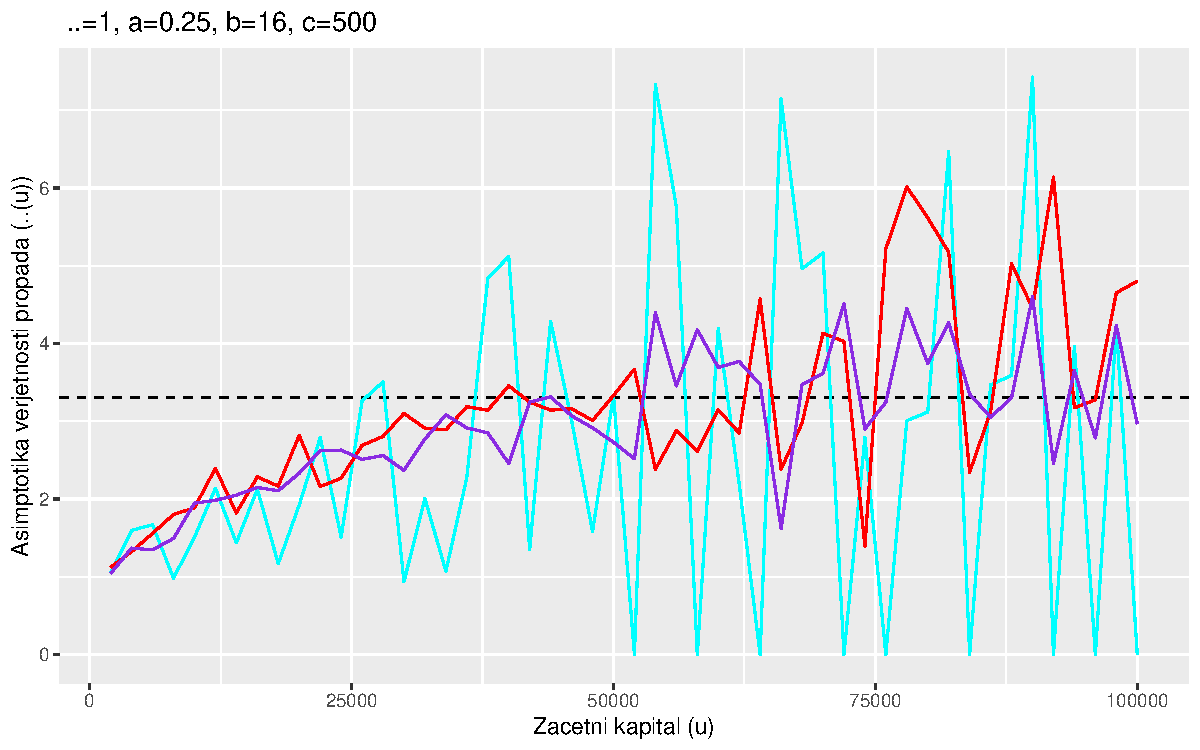
\includegraphics[width=\textwidth]{
                C:/Users/38651/OneDrive - Univerza v Ljubljani/Desktop/Diploma/Diplomski-seminar/GraphsAndPhotos/slika5.pdf
                }
            \caption{Aproksimacija verjetnosti propada $\psi(u)$ z Monte Carlo simulacijami (modra) in 
            to"cna vrednost funkcije (rde"ca).}
            \label{fig:slika5}
        \end{figure}

        \noindent
        Vidimo, da razmerje vizualno res konvergira proti $\tfrac{1}{\rho}$, ampak seveda bi 
        za bolj"so natan"cnost morali pove"cati za"cetni kapital $u$ in "stevilo simulacij. 
        \label{zg:MonteCarloTezkiRepi}
        \end{zgled}

        
        
        





\pagebreak

\section{Priloga}
    Dostavek je namenjen predvsem za dodatne definicije in trditve, ki so bile izpu"scene v glavnem
    za namene preglednosti besedila. V primeru, da bralec potrebuje osve"ziti dolo"cene pojme, 
    jih ve"cino lahko najde v tem razdelku.
    \begin{definicija}
        Naj bo $X$ slu"cajna spremenljivka. Potem so za $u\in\R$ njena \textit{rodovna funkcija}, 
        \textit{momentno rodovna funkcija} in \textit{karakteristi"cna funkcija} definirane 
        kot 
        \begin{equation*}
            G_X(u) = \E\left[u^X\right], \quad M_X(u) = \E\left[e^{uX}\right], \quad \varphi_X(u) = \E\left[e^{iuX}\right],
        \end{equation*}
        "ce upanja obstajajo.
        \label{def:rodovneFunkcije}
    \end{definicija}

    \begin{definicija}
        Naj bo $(\Omega, \mathcal{F}, \Prob)$ verjetnostni prostor. Nara"scajocemu zaporedju 
        $\sigma$-algeber $(\mathcal{F}_t)_{t\geq0}$ pravimo \textit{filtracija}, "ce za vsak $ 0\leq s\leq t$ velja
     $\mathcal{F}_s \subseteq \mathcal{F}_{t} \subseteq \mathcal{F}.$ Za slu"cajni proces $(X_t)_{t\geq0}$ pravimo, 
     da je \textit{prilagojen} filtraciji $\mathcal{F}$, "ce je $X_t$ $\mathcal{F}_t$-merljiva za vsak $t\geq0$.
     \label{def:filtracija}
    \end{definicija}

    \begin{definicija}
        Slu"cajna spremenljivka $X$ ima \textit{Weibullovo porazdelitev} s parametri $a, b > 0$, 
        "ce ima njena porazdelitev obliko 
        \begin{equation*}
            F_X(x) = 1 - e^{-\left(\tfrac{x}{b}\right)^a} \quad \text{za} \ x\geq 0
        \end{equation*}
        in gostota obliko
        \begin{equation*}
            f_X(x) = \left(\frac{a}{b}\right)\left(\frac{x}{b}\right)^{a-1}e^{-\left(\tfrac{x}{b}\right)^a} \quad \text{za} \ x\geq 0.
        \end{equation*}
        \label{def:WeibullovaPorazdelitev}
    \end{definicija}

    \begin{definicija}
        Naj bo $(X_i)_{i\in\N}$ zaporedje neodvisnih enako porazdeljenih slu"cajnih spremenljivk in 
        $G \sim \text{Geom}(p)$ geometrijsko porazdeljena slu"cajna spremenljivka  parametrom $p\in(0, 1)$ in 
        funkcijo verjetnosti $P(G = k) = p(1 - p)^{k}$ za $k\in\N_0$.
        Naj bo $G$ neodvisna od $X_i$ za vsak $i\in\N$. Potem pravimo, da ima slu"cajna spremenljivka
        \begin{equation*}
            C = \sum_{i= 1}^{G} X_i
        \end{equation*}
        \textit{sestavljeno geometrijsko porazdelitev}.
        \label{def:CompoundGeometricDistribution}
    \end{definicija}

    \begin{trditev}
        Naj bo $X$ nenegativna slu"cajna spremenljivka na verjetnostnem prostoru $(\Omega, \mathcal{F}, \Prob)$, 
        ki ima prvi moment. Potem velja 
        \begin{equation*}
            \E\left[X\right] = \int_{(0, \infty)}\bigl(1 - F_X(x)\bigr)dx.
        \end{equation*}
        \label{trd:PricakovanaVrednostZPrezivetveno}
    \end{trditev}

    \begin{proof}
        $X$ lahko zapi"semo kot 
        \begin{equation*}
            X = \int_{(0, \infty)}\mathbbm{1}_{\{x < X\}}dx = \int_{(0, \infty)}\mathbbm{1}_{\{X < x\}}dx.
        \end{equation*}
        "Ce sedaj uporabimo fubinijev izrek dobimo
        \begin{align*}
            \E\left[X\right] &= \E\left[\int_{(0, \infty)}\mathbbm{1}_{\{X < x\}}dx\right] \\
                             &= \int_{(0, \infty)}\E\left[\mathbbm{1}_{\{X < x\}}\right]dx \\
                             &= \int_{(0, \infty)}\bigl(1 - \Prob\left(X > x\right)\bigr)dx \\
        \end{align*}
    \end{proof}

    \begin{trditev}(Neenakost Markova)
        \label{trd:neenakostMarkova}
        Naj bo $X$ nenegativna slu"cajna spremenljivka.
        Potem za  $x>0$ velja
        \begin{equation*}
            \Prob\left(X > x\right) \leq \frac{\E\left[X\right]}{x}.
        \end{equation*}
    \end{trditev}

    \begin{proof}
        Naj bo $x > 0$. Velja
        \begin{equation*}
            x\mathbbm{1}_{\{X > x\}} \leq X \iff x\Prob\left(X > x\right) \leq \E\left[X\right].
        \end{equation*}
    \end{proof}

    \begin{izrek}(Krepki zakon velikih "stevil)
        Naj bo $(X_n)_{n\in\N}$ zaporedje neodvisnih enako porazdeljenih
        slu"cajnih spremenljivk na verjetnostnem prostoru $(\Omega, \mathcal{F}, \Prob)$
         s pri"cakovano vrendostjo $\E\left[X_i\right] = \mu <\infty$. Potem velja
        \begin{equation*}
            \frac{X_1 + X_2 + \cdots X_n}{n}\xrightarrow[n\to\infty]{s.g.} \mu.
        \end{equation*}
        \label{izr:KrepkiZakonVelikihStevil}
    \end{izrek}

    \begin{proof}
        Dokaz izreka lahko bralec najde v \cite{7}.
    \end{proof}

    \begin{izrek}(Izrek o enoli"cnosti)
        Naj bosta $X$ in $Y$ slu"cajni spremenljivki, ne nujno definirani na istem verjetnostnem prostoru.
        "Ce za vsak $u\in\R$ velja $\varphi_X(u) = \varphi_Y(u)$, potem imata $X$ in $Y$ enako porazdelitev.
        \label{izr:enolicnost}
    \end{izrek}

    \begin{proof}
        Dokaz izreka lahko bralec najde v \cite{7}.
    \end{proof}

    \begin{izrek}(Lévijev izrek o kontinuiteti)
        Naj bo $(X_n)_{n\in\N}$ zaporedje slu"cajnih spremenljivk (ne nujno na istem verjetnostnem prostoru)
        in $X$ "se ena slu"cajna spremenljivka. Potem za vsak $u\in\R$ velja
        \begin{equation*}
            \varphi_{X_n}(u) \xrightarrow{n\to\infty} \varphi_X(u) 
        \end{equation*}
        natanko tedaj, ko velja
        \begin{equation*}
            X_n \xrightarrow[n\to\infty]{d} X.
        \end{equation*}
        \label{izr:LevijevIzrek}
    \end{izrek}

    \begin{proof}
        Dokaz izreka lahko bralec najde v \cite{7}.
    \end{proof}

    \begin{izrek}(Lebesgueov izrek o monotoni konvergenci)
        Naj bo $X_1, X_2, \dots $ zaporedje nenegativnih slu"cajnih spremenljivk na 
        verjetnostnem prostoru $(\Omega, \mathcal{F}, \Prob)$ in naj bo $X:= \lim_{n\to\infty}X_n$ 
        njihova limita. Naj za vsak $\omega \in \Omega$
        velja $X_1(\omega) \leq X_2(\omega) \leq \dots$ Potem velja 
        \begin{equation*}
            \lim_{n\to\infty}\E\left[X_n\right] = \E\left[\lim_{n\to\infty}X_n\right] = \E\left[X\right].
        \end{equation*}
        \label{izr:monotonaKonvergenca}
    \end{izrek}

    \begin{proof}
        Dokaz izreka lahko bralec najde v \cite{7}.
    \end{proof}  

    \begin{izrek}(Lebesgueov izrek o dominirani konvergenci)
        Naj bo $X_1, X_2, \dots $ zaporedje slu"cajnih spremenljivk na verjetnostnem prostoru
        $(\Omega, \mathcal{F}, \Prob)$ in naj bo $X:= \lim_{n\to\infty}X_n$ njihova limita.
        Naj bo $Y$ slu"cajna spremenljivka definirana na istem verjetnostnem prostoru z $\E\left[Y\right]<\infty$ in
        naj za vsak $n\in\N$ in vsak $\omega\in\Omega$ velja $|X_n(\omega)| \leq Y(\omega)$. Potem je $X$ integrabilna
        in velja 
        \begin{equation*}
            \lim_{n\to\infty}\E\left[X_n\right] = \E\left[\lim_{n\to\infty}X_n\right] = \E\left[X\right].
        \end{equation*}
        \label{izr:dominiranaKonvergenca}
    \end{izrek}

    \begin{proof}
        Dokaz izreka lahko bralec najde v \cite{7}.
    \end{proof}

    \begin{izrek}(Tonellijev izrek)
        Naj bosta $X$ in $Y$ slu"cajni spremenljivki definirani vsaka na svojem verjentnostnem prostoru
        in naj imata vsaka svojo gostoto $f_X$ in $f_Y$ glede na Lebesgueovo mero.
        Potem velja
        \begin{equation*}
            \int_{\R^2}f_{X, Y}(x, y)\mathcal{L}^2(dx, dy) 
            = \int_{\R}\left(\int_{\R}f_{X, Y}(x, y)dx\right)dy = \int_{\R}\left(\int_{\R}f_{X, Y}(x, y)dy\right)dx.
        \end{equation*}
        \label{izr:TonellijevIzrek}
    \end{izrek}

    \begin{proof}
        Dokaz izreka lahko bralec najde v \cite{7}.
    \end{proof} 

    \begin{trditev}
        Definicija homogenega Poissonovega procesa \ref{def:HPP} je ekvivalentna karakterizaciji 
        z lastnostjo vrstilnih statistik. Naj bo $\lambda > 0$ in $(N_t)_{t\geq0}$ enostavni 
        proces "stetja za katerega je $N_0 = 0$ s.g.\ Naj za vsak $t\geq0$ velja $N_t \sim \text{Pois}(\lambda t)$ in, 
        pogojno na dogodek $\{N_t = k\}$ je vektor "casov prihodov porazdeljen kot 
        \begin{equation*}
            (V_1, \dots, V_k) \mid \{N_t = k\} \sim (U_{(1)}, \dots, U_{(k)}),
        \end{equation*}
        kjer je $(U_{(1)}, \dots, U_{(k)})$ vektor vrstilnih statistik vektorja $(U_1, \dots, U_k)$ 
        neodvisnih \newline enako porazdeljenih slu"cajnih spremenljivk $U_i\sim U\left([0, t]\right)$.
        \label{trd:VrstilneStatistikeHPP}
    \end{trditev}

    \begin{proof}
        Dokaz trditve lahko bralec najde v \cite{7}.
    \end{proof}

    \begin{definicija}
        Naj bo $X$ nenegativna slu"cajna spremenljivka in $F_X$ njena porazdelitvena funkcija. 
        Potem za $u\in\R$ \textit{Laplace-Stiltjesovo transformacijo} porazdelitve $F_X$ definiramo kot
        \begin{equation*}
            \hat{F}_X(u) = \int_{[0, \infty)}e^{-ux}dF_X(x).
        \end{equation*}
        \label{def:LaplaceStiltjesovaTransformacija}
    \end{definicija}

    \begin{definicija}
        Naj bo $F$ porazdelitvena funckija neke nenegativne slu"cajne spremenljivke s prvim 
        momentom. Potem je 
        \begin{align*}
            \overline{F}(x) = \frac{1}{\mathbb{E}[X]} \int_0^x (1 - F(t)) \, dt
        \end{align*}
        \textit{porazdelitev integrarnega repa F}.
        \label{def:porazdelitevintegriranegaRepa}
    \end{definicija}

    \begin{definicija}
        \textit{Prenovitveni proces} na verjentostnem protoru $(\Omega, \mathcal{F}, \Prob)$ je slu"cajni 
        proces
        karatkteriziran z zaporedjem neodvisnih enako porazdeljenih medprihodnih "casov $(T_n)_{n\in\N}$, 
        ki zavzamejo vrednosti v $\R^+\cup\{\infty\}$ in je podan z zvezo 
        \begin{equation*}
            N_t = \sum_{n=1}^{\infty}\mathbbm{1}_{\{S_n\leq t\}},
        \end{equation*}
        kjer je $S_n = T_1 + T_2 + \cdots + T_n$ "cas $n$-tega prihoda. Pripadajo"co 
        \textit{prenovitveno mero} prenovitvenega procesa definiramo kot $M(t) = \E\left[N_t\right]$ za 
        $t > 0$.
        \label{def:PrenovitveniProces}
    \end{definicija}

    \begin{definicija}
        \textit{Prenovitvena ena"cba} je ena"cba oblike 
        \begin{equation*}
            f(t) = g(t) + \int_{[0, t]}f(t - s)dF(s), \quad t\geq 0,
        \end{equation*}
        kjer sta neznana funkcija $f$ in znana funckija $g$ definirani na $\R^+$ in $F$ je 
        porazdelitvna funkcija neke pozitivne slu"cajne spremenljivke $X$. Prenovitveno ena"cbo predstavimo
        s parom $(g, F)$.
        \label{def:prenovitvenaEnacba}
    \end{definicija}

    \begin{definicija}
        Za nenegativno merljivo funkcijo \( f : [0, \infty) \to [0, \infty) \) pravimo, da je \textit{direktno 
        Riemannovo integrabilna} (d.R.i.), če za vsak $\delta > 0$ velja
        \begin{equation*}
            \sum_{k \geq 0} \left( \sup_{t \in [k\delta, (k+1)\delta)} f(t) \right) < \infty \quad \text{in}
        \end{equation*}
        \begin{equation*}
             \lim_{\delta \downarrow 0} \delta \sum_{k \geq 0} \left( \sup_{t \in [k\delta, (k+1)\delta)} f(t) \right) = \lim_{\delta \downarrow 0} \delta \sum_{k \geq 0} \left( \inf_{t \in [k\delta, (k+1)\delta)} f(t) \right).
        \end{equation*}
        Če \(f\) zadošča navedenima zahtevama, potem je limita v drugi zahtevi točno vrednost direktnega Riemannovega integrala
        \[
        \text{d.R.i.} \int_{0}^{\infty} f(t) \, dt.
        \]
        Funkcija \(f\) poljubnega predznaka je d.R.i., če sta le-taki \(f^+ = \max\{f, 0\}\) in \(f^- = \max\{-f, 0\}\), pri čemer je
        \[
        \text{d.R.i.} \int_{0}^{\infty} f(t) \, dt = \text{d.R.i.} \int_{0}^{\infty} f^+(t) \, dt - \text{d.R.i.} \int_{0}^{\infty} f^-(t) \, dt.
        \]
        \label{def:direktnaRieamnovaIntegrabilnost}
    \end{definicija}

    \begin{trditev}(Kriterij za direktno Riemannovo integrabilnost)
        Naj bo $f \geq 0$ nenara"scajo"ca funkcija. Potem je $f$ direktno Riemannovo integrabilna natanko tedaj, ko je
        posplo"seno Riemannovo integrabilna. Tedaj je njen direktni Riemannov integral enak posplo"senemu.
        \label{trd:kriterijZaDirektnoRiemannovoIntegrabilnost}
    \end{trditev}

    \begin{proof}
        Dokaz izreka lahko bralec najde v \cite{8} na strani 235. 
    \end{proof} 

    \begin{izrek}(Smithov klju"cni prenovitveni izrek)
        "Ce je funkcija $g$ iz prenovitvene ena"cbe $(g, F)$ (definicja \ref{def:prenovitvenaEnacba})
        omejena na kon"cnih intervalih in $X$ ima prvi moment ter ni aritmeti"cna 
        $(\nexists a\in\R: \ \Prob\left(X \in \mathbb{Z} a\right) = 1)$, potem je
        \begin{equation*}
            f(t) = g(t) +  \int_{[0, t]}g(t - s)dM(s), \quad t\geq 0,
        \end{equation*}
        enoli"cna re"sitev te ena"cbe. $M(s)$ je prenovitvena mera prenovitvenega procesa z medprihodno 
        porazdelitvijo $F$.
        "Ce je dodatno funkcija $g$ direktno Riemannovo integrabilna velja 
        \begin{equation*}
            \lim_{t\to\infty}f(t) = \frac{1}{\E\left[X\right]}\int_{(0, \infty)}g(t)dt.
        \end{equation*}
        \label{izr:Smith}
    \end{izrek}

    \begin{proof}
        Dokaz izreka lahko bralec najde v \cite{8} na strani 237. 
    \end{proof}

%-----------------------------------------KONEC VSEBINE--------------------------------------------%

\pagebreak
\section*{Slovar strokovnih izrazov}

\noindent
\textbf{trajektorija} \ sample path \\
\textbf{slu"cajni proces} \ stochastic process \\
\textbf{sestavljeni Poissonov proces} \ compound Poisson process \\
\textbf{neskon"cna deljivost} \ infinite divisibility \\
\textbf{proces tveganja} \ risk process \\
\textbf{verjetnost propada} \ probability of ruin \\
\textbf{ogrodje procesa tveganja} \ skeleton process \\
\textbf{lahkorepa porazdelitev} \ light-tailed distribution \\
\textbf{te"zkorepa porazdelitev} \ heavy-tailed distribution \\
\textbf{subeksponentna porazdelitev} \ subexponential distribution \\
\textbf{prenovitveni proces} \ renewal process \\
\textbf{defektna prenovitvena ena"cba} \ defective renewal equation \\
\textbf{prenovitvena mera} \ renewal function \\

% Literatura
\begin{thebibliography}{99}
\bibitem{1}S.E. Shreve, Stochastic Calculus for Finance II: Continuous-Time Models, Springer, (2004).
\bibitem{2}S.M. Ross, Stochatic Processes: Second Edition, Wiley, (1996).
\bibitem{3}P. Embrechts, C. Klüppelberg, T. Mikosch, Modelling Extremal Events: For Insurance and Finance, Springer, (1997).
\bibitem{4}T. Mikosch, Non-Life Insurance Mathematics: An Introduction with the Poisson Process, Second Edition, Springer, (2009).
\bibitem{5}M. Mandjes, O. Boxma, The Cramér--Lundberg model and its variants, Springer, (2023).
\bibitem{6}F. Spitzer, Principles of Random Walk. Second Edition, Springer, (1976).
\bibitem{7}B. Fristedt, L. Gray, A Modern Approach to Probability Theory, Springer, (1996).
\bibitem{8}S.I. Resnick, Adventures in Stochastic Processes, Birkhäuser, (1992).
\bibitem{9}R.J. Adler, R.E. Feldman, A practical guide to heavy tails: statistical techniques and applications, Birkhäuser, (1998).
\end{thebibliography}

\end{document}